\NeedsTeXFormat{LaTeX2e}
\documentclass[12pt, a4paper]{book}

\usepackage[sc]{mathpazo}
\linespread{1.05}
\usepackage[Lenny]{fncychap}
\usepackage{fancyhdr}
\usepackage[utf8]{inputenc}
\usepackage{blindtext}
\usepackage{tikz}
\usetikzlibrary{shapes, arrows}
\usepackage{tikz-3dplot}
\usepackage{epsfig}
\usepackage{epstopdf}
\usepackage{graphicx}
\usepackage{caption}
\usepackage{subcaption}
\usepackage{keyval}
\usepackage{float}
\usepackage{listings}
\usepackage{color}
\usepackage{textcomp}
\usepackage{datetime}
\usepackage[numbers, sort&compress, comma]{natbib}
\usepackage{subeqnarray}
\usepackage{longtable}
\usepackage{booktabs}
\usepackage{array}
\usepackage{amsmath}
\usepackage{amsfonts}
\usepackage{amssymb}
\usepackage [linktocpage=all]{hyperref}
\hypersetup{
  pdftitle    = {Titel},
  pdfsubject  = {Electrical Engineering},
  pdfauthor   = {Robin Weiß},
  pdfkeywords = {Bachelor Thesis} ,
  pdfcreator  = {pdflatex},
  pdfproducer = {LaTeX}
}

\usepackage[acronym, nopostdot, nonumberlist]{glossaries}
\newglossary[nlg]{notation}{not}{ntn}{Notation}

\setcounter{tocdepth}{3}
\setcounter{secnumdepth}{4}

\lhead[\fancyplain{}{\thepage}]{\fancyplain{}{\sl\nouppercase\rightmark}}
\rhead[\fancyplain{}{\sl\nouppercase\leftmark}]{\fancyplain{}{\thepage}}
\cfoot{}

\clubpenalty = 10000
\widowpenalty = 10000 
\displaywidowpenalty = 10000

\newcommand{\clearemptydoublepage}
{\newpage{\pagestyle{empty}\cleardoublepage}}

\makeglossaries
\setlength{\glsdescwidth}{0.8\linewidth}


\newacronym{CITIC-UGR}{CITIC-UGR}{Research Centre for Information and Communications Technologies of the University of Granada}

\newacronym[description=Inertial measurement unit]{IMU}{IMU}{inertial measurement unit}

\newacronym[description=Magnetic inertial measurement unit]{MIMU}{MIMU}{magnetic inertial measurement unit}

\newacronym[description={Magnetic, angular rate, and gravity sensors}]{MARG}{MARG sensors}{Magnetic, angular rate, and gravity sensors}

\newacronym[description={Microelectromechanical systems}]{MEMS}{MEMS}{microelectromechanical systems}

\newacronym[description={Angle random walk}]{ARW}{ARW}{angle random walk}


\newglossaryentry{not:F}{
  type=notation,
  name={$\mathbf{F}$},
  description={Three-dimensional force vector},
  sort={F}}
  
\newglossaryentry{not:B_v}{
  type=notation,
  name={$\mathbf{B}$},
  description={Control matrix that relates the control input to the state $\mathbf{x}$},
  sort={Ba}}
 
\newglossaryentry{not:m}{
  type=notation,
  name={$m$},
  description={Mass},
  sort={m}}
  
\newglossaryentry{not:sigma}{
  type=notation,
  name={$\sigma$},
  description={Standard deviation},
  sort={sigma}}
  
\newglossaryentry{not:sigma_2}{
  type=notation,
  name={$\sigma^2$},
  description={Variance},
  sort={sigma}}
  
\newglossaryentry{not:mu}{
  type=notation,
  name={$\mu$},
  description={Mean value of conditional probability density},
  sort={sigma}}
  
\newglossaryentry{not:n}{
  type=notation,
  name={$n$},
  description={Discrete time},
  sort={n}}
  
\newglossaryentry{not:a}{
  type=notation,
  name={$\mathbf{a}$},
  description={Three-dimensional acceleration vector},
  sort={a}}
  
\newglossaryentry{not:impulse}{
  type=notation,
  name={$w_0, w_1, w_2, \dots$},
  description={Impulse response of a linear discrete-time filter},
  sort={wa}}
  
\newglossaryentry{not:input}{
  type=notation,
  name={$y(0), y(1), y(2), \dots$},
  description={Time series that serves as input to a linear discrete-time filter},
  sort={yaa}}
  
\newglossaryentry{not:desired_response}{
  type=notation,
  name={$d$},
  description={Desired filter response of a linear discrete-time filter},
  sort={d}}
  
\newglossaryentry{not:error_signal}{
  type=notation,
  name={$e$},
  description={Error signal of a linear discrete-time filter},
  sort={e}}
  
\newglossaryentry{not:t}{
  type=notation,
  name={$t$},
  description={Continuous time},
  sort={t}}

\newglossaryentry{not:x_v}{
  type=notation,
  name={$\mathbf{x}$},
  description={State vector of a linear dynamical system},
  sort={xb}}
  
\newglossaryentry{not:x}{
  type=notation,
  name={$x$},
  description={One-dimensional location},
  sort={x}}
  
\newglossaryentry{not:x_hat}{
  type=notation,
  name={$\hat{x}$},
  description={Estimate of $x$},
  sort={xa}}
  
\newglossaryentry{not:w_v}{
  type=notation,
  name={$\mathbf{w}$},
  description={Process noise vector},
  sort={wa}}
  
\newglossaryentry{not:v}{
  type=notation,
  name={$\mathbf{v}$},
  description={Measurement noise vector},
  sort={v}}
  
\newglossaryentry{not:u}{
  type=notation,
  name={$u$},
  description={Nominal velocity},
  sort={u}}
  
\newglossaryentry{not:w}{
  type=notation,
  name={$w$},
  description={Noise term},
  sort={w}}

\newglossaryentry{not:x_hat_v}{
  type=notation,
  name={$\hat{\mathbf{x}}$},
  description={Estimate of the state vector of a linear dynamical system},
  sort={xd}}
  
\newglossaryentry{not:x_hat_minus}{
  type=notation,
  name={$\hat{\mathbf{x}}^-_k$},
  description={A priori estimate of $\hat{\mathbf{x}}$, conditioned on all prior measurements except the one at time $t_k$},
  sort={xe}}
  
\newglossaryentry{not:y}{
  type=notation,
  name={$\mathbf{y}$},
  description={Observation vector of a dynamical system},
  sort={y}}
  
\newglossaryentry{not:z}{
  type=notation,
  name={$\mathbf{z}$},
  description={Vector of measured values},
  sort={zaa}}
  
\newglossaryentry{not:H}{
  type=notation,
  name={$\mathbf{H}$},
  description={Measurement sensitivity matrix defining the linear relationship between the state of the dynamical system and the measurements that can be made},
  sort={Ha}}
  
\newglossaryentry{not:K_v}{
  type=notation,
  name={$\mathbf{K}$},
  description={Kalman gain matrix},
  sort={Kaa}}
  
\newglossaryentry{not:K}{
  type=notation,
  name={$K$},
  description={Weighting factor},
  sort={Ka}}
  
 \newglossaryentry{not:k}{
  type=notation,
  name={$k$},
  description={Discrete time normalised to sampling interval (sample number), $k \in \mathbb{N}^0$},
  sort={k}}
  
\newglossaryentry{not:P}{
  type=notation,
  name={$\mathbf{P}$},
  description={Covariance matrix of state estimation uncertainty},
  sort={P}}
  
\newglossaryentry{not:Q}{
  type=notation,
  name={$\mathbf{Q}$},
  description={Covariance matrix of process noise in the system state dynamics},
  sort={Q}}
  
\newglossaryentry{not:R}{
  type=notation,
  name={$\mathbf{R}$},
  description={Covariance matrix of observational (measurement) uncertainty},
  sort={R}}
  
\newglossaryentry{not:phi}{
  type=notation,
  name={$\bm{\Phi}$},
  description={State transition matrix of a discrete linear dynamical system},
  sort={phiaa}}
  
\newglossaryentry{not:x_k}{
  type=notation,
  name={$\mathbf{x}_k$},
  description={The $k$th element of a sequence $\dots$, $\mathbf{x}_{k-1}$, $\mathbf{x}_k$, $\mathbf{x}_{k+1}, \dots$ of vectors},
  sort={xc}}
  
 \newglossaryentry{not:unit-delay}{
  type=notation,
  name={$z^{-1}$},
  description={Unit-delay},
  sort={za}}
  
\newglossaryentry{not:roll}{
  type=notation,
  name={$\phi$},
  description={Roll angle that determines the rotation around the $x$-axis},
  sort={phi}}
  
\newglossaryentry{not:pitch}{
  type=notation,
  name={$\theta$},
  description={Pitch angle that determines the rotation around the $y$-axis},
  sort={theta}}
  
\newglossaryentry{not:yaw}{
  type=notation,
  name={$\psi$},
  description={Yaw angle that determines the rotation around the $z$-axis},
  sort={psi}}

\newglossaryentry{not:navigation_frame}{
  type=notation,
  name={$x, y, z$},
  description={Axes of the fixed navigation frame},
  sort={xayaza}}
  
\newglossaryentry{not:body_frame}{
  type=notation,
  name={$X, Y, Z$},
  description={Axes of the moving body frame},
  sort={xayazb}}
  
\newglossaryentry{not:transformation_matrix}{
  type=notation,
  name={$\mathbf{T}$},
  description={Transformation matrix},
  sort={Ta}}
  
\newglossaryentry{not:transformation_matrix_bn}{
  type=notation,
  name={$\mathbf{C}_{bn}$},
  description={Transformation matrix transforming a position vector from the body frame to the navigation frame},
  sort={Cbn}}
  
\newglossaryentry{not:transformation_matrix_nb}{
  type=notation,
  name={$\mathbf{C}_{nb}$},
  description={Transformation matrix transforming a position vector from the navigation frame to the body frame},
  sort={Cnb}}
  
\newglossaryentry{not:omega}{
  type=notation,
  name={$\bm{\Omega}_{\mathbf{E} \rightarrow \mathbf{E}}$},
  description={Function that transforms a position vector $\mathbf{b}$ in the vector space $\mathbf{E}$ into the vector $\mathbf{b}^{'}$ in the vector space $\mathbf{E}^{'}$},
  sort={Om}}
  
\newglossaryentry{not:position_vector}{
  type=notation,
  name={$\mathbf{b}$},
  description={Position vector in a three-dimensional vector space},
  sort={b}}
  
\newglossaryentry{not:phi_vec}{
  type=notation,
  name={$\bm{\phi}$},
  description={Functional denoting the \emph{non-linear} transition matrix function of a discrete dynamical system},
  sort={phia}}
  
\newglossaryentry{not:h_vec}{
  type=notation,
  name={$\mathbf{h}$},
  description={Functional denoting the \emph{non-linear} measurement matrix function of a discrete dynamical system},
  sort={h}}
  
  

% Add all glossary entries not only the referenced ones.
\glsaddall
    

\begin{document}

	\frontmatter

	\begin{titlepage}
\label{ch:titlepage}
\begin{center}


\includegraphics[width=7cm]{images/universidad_de_granada.eps}
	\hfill

\includegraphics[width=5cm]{images/fh-muenster.eps}
	\hspace{1.0cm}
	\\ 

\vspace{3cm}

\Large\textbf{Bachelor Thesis}

\large\textsc{electrical engineering}

\vspace{1cm}

{\huge\textbf{Analysis of Anticipatory Postural Adjustments of Parkinson's Patients Using Inertial Sensors}}

\vspace{1cm}

Department of Electrical Engineering and Computer Science

\textbf{Münster University of Applied Sciences}

\end{center}

\vspace{1.5cm}

\textbf{Written by:}  \hfill \textbf{Supervised by:}

Robin Weiß \hfill Prof. Dr.-Ing. Peter Gl\"{o}sek\"{o}tter 

\hfill Ph.D. Alberto Olivares Vicente

\hfill Prof. Dr. med. Kai B\"{o}tzel

\vfill

Granada, \today

\end{titlepage}

	\clearemptydoublepage
	
	\setcounter{page}{1}	
	\phantomsection
	\addcontentsline{toc}{chapter}{Statement of Authorship}
	\thispagestyle{empty}

\section*{Statement of Authorship}
I hereby certify that this bachelor thesis has been composed by myself, and describes my own work, unless otherwise acknowledged in the text. All references and verbatim extracts have been quoted, and all sources of information have been specifically acknowledged. It has not been accepted in any previous application for a degree.

\vspace{1cm}

\noindent 
Granada, \the\day st \monthname \: \the\year

\vspace{2cm}

\noindent
Robin Weiß

	\clearemptydoublepage
	
	\phantomsection
	\addcontentsline{toc}{chapter}{Preface}
	\chapter{Preface}

This thesis was submitted in partial fulfilment of the requirements for the degree of Bachelor of Science in Electrical Engineering. It describes the implementation of a new Kalman filter based orientation algorithm to improve the estimation of orientation angles by means of inertial sensors.

I took part in the joint research project “Human Body Motion Analysis of Patients with Neurodegenerative Diseases by Means of Inertial Sensors” between the \gls{CITIC-UGR}, Spain, and the Department of Neurology of the Klinikum Großhadern, which is part of the Ludwig Maximilian University of Munich, Germany. The goal of the overall project was to obtain several gait parameters by wearable inertial sensors and validate them against conventional methods such as force plates and cameras in combination with visual markers. Physicians and medical researchers are interested in this approach of body motion analysis, as unobtrusive wearable sensors can assist the diagnosis of neurodegenerative diseases such as Parkinson's. Prior to this thesis I completed a three-months internship at the \gls{CITIC-UGR} in which I worked on the synchronisation of a force measuring plate and inertial sensors within the above-mentioned project.
	\clearemptydoublepage

	\phantomsection
	\addcontentsline{toc}{chapter}{Abstract}
	\thispagestyle{plain}
  \null\vfil
  
\begin{center}
    \setlength{\parskip}{0pt}
    {\normalsize \textsc{Münster University of Applied Sciences} \par}
    \bigskip
    {\huge{\textsc{Abstract}} \par}
    \bigskip
    {\normalsize Department of Electrical Engineering and Computer Science \par}
    \bigskip
    {\normalsize Bachelor of Science \par}
    \bigskip
    {\normalsize\bf Analysis of anticipatory postural adjustments of Parkinson's patients using inertial sensors \par} % Thesis title
    \medskip
    {\normalsize by Robin Weiß \par} % Author name
    \bigskip
  \end{center}

\noindent  
This thesis entitled ``Analysis of anticipatory postural adjustments of Parkinson's patients using inertial sensors'' was submitted in partial fulfilment of the requirements for the degree of Bachelor of Science in Electrical Engineering. 

I took part in a conjoint project between the Research Centre for Information and Communications Technologies of the University of Granada (CITIC-UGR) and the Department of Neurology of the Klinikum Großhadern in Munich, which is part of the Ludwig-Maximilians University. The objective of this thesis was to carry out an analysis of the so called anticipatory postural adjustments, which are the movements by a human subject between the moment he initiates gait and the first step.



	\clearemptydoublepage
	
	\phantomsection
	\addcontentsline{toc}{chapter}{Contents}
	\tableofcontents
	\thispagestyle{plain}
		
	\listoffigures
	\phantomsection
	\addcontentsline{toc}{chapter}{List of Figures}
	\thispagestyle{plain}
	\clearemptydoublepage

	\listoftables
	\phantomsection
	\addcontentsline{toc}{chapter}{List of Tables}
	\thispagestyle{plain}
	\clearemptydoublepage	
	
	\printglossary[type=acronym, title={Abbreviations}, style=super]
	\phantomsection
	\addcontentsline{toc}{chapter}{Abbreviations}
	\thispagestyle{plain}
	\clearemptydoublepage
    
    \printglossary[type=notation, style=super]
    \phantomsection
    \addcontentsline{toc}{chapter}{Notation}
    \thispagestyle{plain}
    \clearemptydoublepage
	
	\mainmatter
	
	\pagestyle{fancyplain}
		
	\chapter{Introduction}
\label{ch:Introduction}

\section{General}

\subsection{Parkinson's Disease}

According to Patients Medical \cite{patients_medical_definition_2014}, \begin{quote}``Parkinson's disease is a progressive, neurodegenerative disease that occurs when the neurons within the brain responsible for producing the chemical dopamine become impaired or die. Dopamine is essential for the smooth control and coordination of the movement of voluntary muscle groups. Once approximately 80\% of the brain's dopamine producing cells no longer function, the symptoms of Parkinson's disease begin to appear. [\dots] Parkinson's disease may be termed as a progressive movement disorder that is distinguished by marked slow movements, tremors, and unstable posture.''\end{quote}

Especially in advanced stages of the Parkinson's disease (PD)\nomenclature{PD}{Parkinson's disease} many patients exhibit an episodic, brief inability to step that delays gait initiation or interrupts ongoing gait. This phenomenon is called freezing of gait and is often associated with an alternating shaking of the knees, called knee trembling. However, these clinical signs of balance or gait problems are not evident in early stages of the disease \cite{mancini_anticipatory_2009}\cite{jacobs_knee_2009}.

\subsection{Anticipatory Postural Adjustments}

A major challange to the human ballance control system is the fact that we are bipeds having only one foot in contact with the ground while walking, and that two-thirds  of our body mass is located two-thirds of body height above the ground \cite{halliday_initiation_1998}. Thus, to induce stable gait anticipatory postural adjustments (APAs)\nomenclature{APAs}{Anticipatory Postural Adjustments} are necessary. The Encyclopedia of Neuroscience \cite[p.133]{woollacott_anticipatory_2009} defines APAs as "A predictive motor response that acts to counter, in a preemptive manner, the postural destabilization associated with a forthcoming movement." As seen in Figure \ref{fig:APAoverview} the centre of body mass (COM)\nomenclature{COM}{Centre of Mass} is accelerated forward and laterally over the stance foot to make sure that the body does not fall laterally toward the stepping foot during the swing phase \cite{woollacott_anticipatory_2009}.  The curve of the centre of pressure (COP)\nomenclature{COP}{Centre of Pressure} is divided in three periods. Period S1 indicates the uncoupling of the COP and COM as the COP moves posteriorly and toward the intended stepping limb. Then, in the S2 period, the COP displaces mediolaterally toward the stance foot. Finally, during the S3 period the COP moves anteriorly under the stance foot \cite{hass_gait_2005-1}.

\begin{figure}
	\centering
	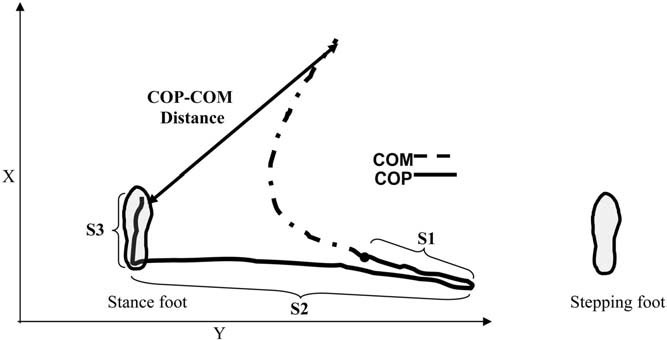
\epsfig{file=images/APA_overview, width=9cm}
	\caption{Anticipatory Postural Adjustments during forward-oriented gait initiation when stepping with the right foot \cite{hass_gait_2005-1}.}
	\label{fig:APAoverview}
\end{figure}


\section{Goals}

The goal of the project was to analyse anticipatory postural adjustments prior to step inition and subsequently build a classifier using MATLAB, which is fed with data from both a force plate and a magnetic inertial measurement unit (GaitWatch \cite{olivares_vicente_gaitwatch_2013}) to distinguish between Parkinson patients and healthy subjects. To gather the data the subject stood in front of the force plate. Then the GaitWatch and force plate record was started and the subject made a step onto the force plate. After standing a variable time of two to ten seconds the subject left the force plate, made a few steps, turned left und stopped in front of it again. This sequence was repeated ten times.


\section{Motivation}

Advanced PD can increasingly diminish quality of life, since patients are dependent on help from others to accomplish daily tasks. New drugs are currently being developed and are expected to decelerate or stop the course of the disease in early stages \cite{botzel_motivation_2014}. Thus, a quantitative PD classification enabling early diagnosis of the disease could optimise early treatment and could help to validate new treatment methods. Additionally, an objective evaluation of longterm treatment success was ensured.


\section{State of the art}

There are several methods and devices to assess Parkinson's disease and to analyse anticipatory postural adjustments. They differ in terms of practicability, accuracy, validity, portability, and cost. The state of the art at the beginning of the project is described below.

\subsection{Rating scales}

A commonly used rating scale is the Unified Parkinson’s Disease Rating Scale (UPDRS),\nomenclature{UPDRS}{Unified Parkinson’s Disease Rating Scale} which is a short test performed by a physician \cite{klerk_long-term_2009}. The patient is rated on 31 different items (see Table \ref{tab:UPDRS}) with a score of 0 (normal) to 4 (severely affected). Another method is the rough, but widely utilised and accepted Hoehn and Yahr scale (HY)\nomenclature{HY}{Hoehn and Yahr scale}. Parkinsonian motor impairment is categorised in 5 stages: Unilateral (Stage 1) to bilateral disease (Stage 2) without balance difficulties, to the presence of postural instability (Stage 3), loss of physical independence (Stage 4), up to being wheelchair- or bed-bound (Stage 5) \cite{goetz_movement_2004}. Without the need of complex technical devices these tests are relatively simple to perform. \citeauthor{klerk_long-term_2009} \cite{klerk_long-term_2009} mentioned their disadvantages, including subjectivity, short observation periods, and unfamiliarity of the environment that both rating methods bring along.

\begin{table}[h]
\begin{tabular}{lll}
\hline
Mentation, mood & Activities of daily & Motor examination \\
and behavior & living & \\
\hline
Intellectual impairment & Speech & Speech \\

Thought disorder & Salivation & Facial expression\\

Depression & Swallowing & Tremor at rest \\

Motivation/initiative & Handwriting & Action or postural tremor of hands \\

& Use of eating utensils & Rigidity \\

& Dressing & Finger taps\\

& Hygiene & Hand movements\\

& Turning in bed & Rapid alternating movements of hands\\

& Falling & Food agility\\

& Freezing when walking & Arising from chair \\

& Walking & Posture\\

& Tremor & Gait\\

& Sensory Complaints & Posture stability\\

& & Body bradikinesia and hypokinesia \\
\hline
\end{tabular}
\caption{Unified Parkinson's Disease Rating Scale items adapted from \cite{herndon_handbook_2006}.}
\label{tab:UPDRS}
\end{table}

\subsection{Instrumentation}

In addition to the aforementioned subjective rating scales, there are different devices used to quantify gait and posture and assess them objectively. All of them come with certain pros and cons. The following devices have been used:

\subsubsection{Electromyographs} Electromyography is a technique for evaluating the electrical activity of skeletal muscles. Successive action potentials generated by muscle cells are measured, by means of needle electrodes inserted into the muscles, and displayed on a cathode-ray oscilloscope. Thus medical abnormalities can be detected. The instrument used to capture the visual recording, termed electromyogram, is called electromyograph \cite{encyclopedia_britannica_electromyography_2014}. Electromyography is constrained to clinical application only, but gives indication about the contribution of specific, individual muscles to APAs.

\subsubsection{Force plates} Force plates quantify the ground reaction force (GRF)\nomenclature{GRF}{Ground Reaction Force}, which is the force exerted to the human body by the ground. The GRF is a three-dimensional vector with three orthogonal components. One component along the direction of gravity, one parallel to the ground in the sagittal plane, and one parallel to the ground in the frontal plane. Those are vertical planes that divide the body in left and right halves, and ventral and dorsal sections, respectively. A force plate usually gives an electrical voltage proportional to the force in each of the three directions. Force plates can be characterised according to the following criteria: Sensitivity in Volts per Newton, crosstalk (indication of vertical force if a horizontal force is applied and vice versa), repeatability (similar results under the same load), and time- and temperature drift \cite{griffiths_principles_2006}. Froce plates are limited to clinical application, too. They have the advantage that they don't have to be calibrated.

\subsubsection{Inertial measurement units} Devices that use a combination of inertial sensors like accelerometers and gyroscopes are referred to as inertial measurement units (IMUs)\nomenclature{IMU}{Inertial Measurement Unit}. If they also include magnetic field sensors (magnetometers), they are called magnetic inertial measurement units (MIMUs)\nomenclature{MIMU}{Magnetic Inertial Measurement Unit}. With these devices the orientation of the body can be obtained with up to nine degrees of freedom, provided that triaxial accelerometers and magnetometers are used, respectively \cite{olivares_vicente_signal_2013}.

\begin{itemize}

\item \textsc{Accelerometers} measure the acceleration of an object relative to an inertial frame. Since acceleration cannot be measured directly, the force exerted to a reference mass is obtained and the resultant acceleration is computed according to Newton's second law $ \mathbf{F} = m \cdot \mathbf a $ \cite{encyclopedia_britannica_accelerometer_2014}.

\item \textsc{Gyroscopes} measure angular velocity and are based on the Coriolis Effect. By means of integration of the angular velocity the rotation angle is obtained \cite{olivares_vicente_signal_2013}.

\item \textsc{Magnetometers} measure the strength and the direction of the magnetic field in a point in space, using the relationship between magnetic fields, movement and induced currents \cite{olivares_vicente_signal_2013}.
 
\end{itemize}
MIMUs are portable and relatively inexpensive. They can be easily attached to the body and thus allow non-clinical longterm application. Their drawbacks are complex calibration procedures and drift behaviour over time, depending on intensity and duration of the movement. Hence, in order to maintain a satisfactory degree of precision, periodical recomputation of the calibration parameters is required \cite{olivares_vicente_signal_2013}.

\subsection{Classification}

There are several research works in the literature dealing with APA analysis and PD classification, as the evaluation of posture and gait are key components of the clinical evaluation of PD \cite{palmerini_classification_2013}.

\citeauthor{klerk_long-term_2009} \cite{klerk_long-term_2009} developed a measurement system called PD Monitor, implementing an Activity Classifier that quantifies tremor and bradykinesia in the arm, thigh, and trunk, in an ambulant way and over long periods of time. They validated their measurements with video records, which were rated by physicians using the UPDRS and concluded that ``the PD monitor can be used for a detailed evaluation of the PD motor symptoms in order to optimize treatment.'' \cite{klerk_long-term_2009}.

\citeauthor{mancini_anticipatory_2009} \cite{mancini_anticipatory_2009} found that the 11 untreated early-to-middle stage Parkinson's patients that took part in their study have a significantly smaller peak COP displacement towards the stepping leg and peak trunk acceleration towards the stance leg compared to the 12 age-matched healthy control subjects. Even though step velocity and step length were not different. The results show that lateral APAs are impaired in early, untreated PD and that they are detectable with inertial sensors. As well as force plate-based, also acceleration-based extracted features can be used to detect impairments equally well. Due to the fact that the acceleration signal can be easily obtained via a sensor on a belt, no matter if in clinical or home environment, APA detection by means of accelerometers is considered as a useful way to characterise patients in early stage of PD without evident clinical symptoms. Additionally in \cite{mancini_anticipatory_2009} it is proposed to carry out further studies to determine the relationship between small APAs and the probability to develop start hesitation and freezing.

\citeauthor{palmerini_classification_2013} \cite{palmerini_classification_2013} states that PD classfication could deliver a tool to follow the progression of the disease during the entire course to examine the efficiency of treatment. They studied classification of PD subjects  using triaxial accelerometers on the lower back at L5 level and an ad hoc wrapper feature selection technique and achieved satisfactory accuracy of 93.75\%. Twenty early-mild PD subjects and 20 healthy age-matched control subjects had to perform two simple tests (quiet standing, Timed Up and Go test), in two evaluations over a 1-year follow-up, to test accuracy and robustness over time. As well as \cite{mancini_anticipatory_2009} they found that lateral dynamics i.e. range of motion are impaired in early-mild PD and suggested further investigation on validity of measures in later stages.

\section{Document structure}


	\chapter{MARG Sensors}
\label{ch:MARG}

MARG sensors is a collective term for magnetic, angular rate, and gravitational sensors, which encompasses inertial sensors, as well as magnetic field sensors, also referred to as magnetometers. Inertial sensors itself generally fall into two categories: instruments sensing linear inertial displacement (accelerometers) and rotational inertial rate sensors (gyroscopes). They are applied in various contexts to quantify vibration, motion, and shock \cite{bhattacharyya_inertial_sensors_applications_13}. Particularly, the development of \gls{MEMS} opened up many medical applications as stated in Section \ref{sec:MARG_sensors_medical}. They have low manufacturing costs, small physical size, and low power consumption \cite{bhattacharyya_inertial_sensors_applications_13}. This chapter compiles the functional principles of MARG sensors and introduces \glspl{IMU} as a combination of those. At the end of the chapter the aforementioned GaitWatch device that was used to gather the movement data for the experiments is described in detail.

\section{Accelerometers}

Accelerometers measure the acceleration of an object relative to an inertial frame. Since acceleration cannot be sensed directly, the force exerted on a reference mass is measured. The resultant acceleration is computed according to Newton's second law $\mathbf{f} = m \cdot \mathbf{a}$, where $ \mathbf{f} \in \mathbb{R}^3$ denotes the force vector, $m$ the mass, and $\mathbf{a} \in \mathbb{R}^3$ the acceleration vector. Usually, an accelerometer consists of a small proof mass connected via a spring to the case of the instrument. The proof mass is displaced  by $\Delta x$ with respect to the case, when the instrument experiences a certain acceleration along its sensitive axis. Disregarding drag force, the displacement is directly proportional to the force exerted by the mass and thus to the acceleration. Therefore, by measuring the displacement of the proof mass the acceleration can be obtained. Figure \ref{fig:accelerometer} shows the displacement $\Delta x$ of the mass in respect to the case of the instrument for three different conditions: (a) at rest or in uniform motion, (b) accelerating, and (c) at rest, being exposed to the gravity $g$. According to how the mass displacement is sensed, accelerometers can be classified as resistive, capacitive, and piezoelectric. Besides, there are surface acoustic wave, fibre optic, vibrating beam and solid-state \gls{MEMS} accelerometers. To obtain a three-dimensional accelerometer, three single-axis accelerometers are mounted together. Although a mutually orthogonal mount is common practice, any non-coplanar arrangement is acceptable, as long as the angles between the sensitive axes are known. Nowadays most accelerometers are manufactured using MEMS technology, which was developed for the military and aerospace markets in the 1970s \cite{bhattacharyya_inertial_sensors_applications_13}. 

\begin{figure}
\centering
\begin{tikzpicture}[scale=0.95, auto, thick, node distance=3cm,>=latex']
    \pgftext{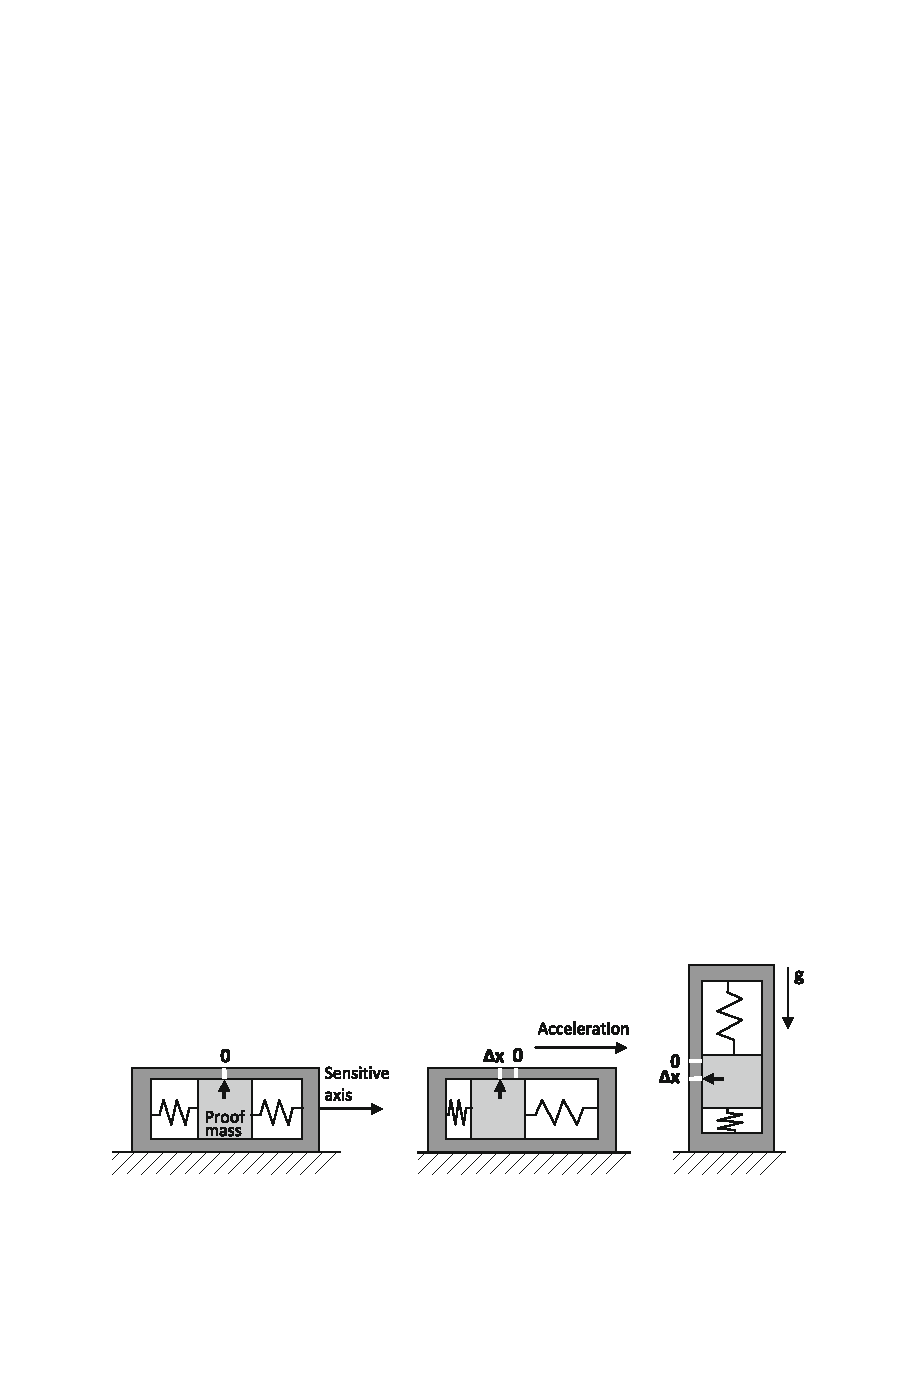
\includegraphics[width=13.5cm]{images/accelerometer}} at (0pt,0pt);
    \node [] (a) at (-6.7, -1.1) {(a)};
    \node [] (b) at (-1.1, -1.1) {(b)};
    \node [] (c) at (3.9, -1.1) {(c)};
    \node [] (c) at (-4.525, 0.44) {$0$};
    \node [] (c) at (1.03, 0.44) {$0$};
    \node [] (c) at (4, 0.26) {$0$};
    \node [] (c) at (0.58, 0.44) {$\Delta x$};
    \node [] (c) at (3.82, -0.08) {$\Delta x$};
    \node [] (c) at (6.5, 1.5) {$\mathbf{g}$};
    \node [] (c) at (-4.525, -0.75) {\scriptsize Proof};
    \node [] (c) at (-4.525, -1.05) {\scriptsize mass};
    \node [] (c) at (-2, -0.05) {\scriptsize Sensitive};
    \node [] (c) at (-2, -0.45) {\scriptsize axis};
    \node [] (c) at (2.2, 0.85) {\scriptsize Acceleration};
\end{tikzpicture}
\caption{A mass-and-spring accelerometer under different conditions: (a) at rest or in uniform motion, (b) accelerating, and (c) at rest, being exposed to the gravity $\mathbf{g}$, from \cite{bhattacharyya_inertial_sensors_applications_13}.}
	\label{fig:accelerometer}
\end{figure}


\section{Gyroscopes}

Gyroscopes are used for measuring and maintaining angular orientation. In essence, based on two different physical principles, namely the Sagnac and Coriolis effect, gyroscopes sense angular velocity, which is why they are also referred to as angular velocity sensors or angular rate sensors. By integrating the angular velocity the rotation angle can obtained. Here we will only elaborate on the working principle of vibrating gyroscopes, since they are utilised in the GaitWatch device. \citeauthor{armenise2010advances} give a comprehensive overview of current gyroscope technologies in \cite{armenise2010advances}.

Coriolis vibratory gyroscopes, or vibrating gyros for short, sense angular velocity based on the effect of Coriolis force on a vibrating mass. The Coriolis force is a fictitious force experienced by a mass $m$ moving in a rotating reference frame. It can be calculated as: $\mathbf{f}_C = -2m(\bm{\omega} \times \mathbf{v})$, where $\mathbf{v}$ is the mass velocity in the rotating reference frame and $\bm{\omega}$ is the angular velocity of the reference frame. As seen in this equation the Coriolis force is only present when the mass varies its distance with respect to the spin axis. Otherwise, if $\bm{\omega}$ and $\mathbf{v}$ are parallel, the cross product becomes zero. The two degree-of-freedom spring-mass-damper system shown in Figure \ref{fig:gyroscope} serves as a simple model of a vibrating angular rate sensor. The mass $m$ can move along the $x$ and $y$-axis, respectively. The angular velocity around the $z$-axis is denoted with $\omega$. The drive or primary oscillating mode, that is, the oscillation along $x$, is excited by the force $F_x$ directed along the $x$-axis. The oscillation along $y$, called sense or secondary oscillating mode, is due to system rotation around the $z$-axis. $D_x$ and $D_y$ are the damping coefficients and $k_x$ and $k_y$ are the spring constants along the $x$ and $y$-axis, respectively. Typically, the primary oscillating mode is excited by a sinusoidal force with an angular frequency close to the resonance frequency, so that $\Omega_x \cong \sqrt{k_x/m}$. Its amplitude is kept constant at $a_x$. As shown in \cite{armenise2010advances},the amplitude of the sense mode is then given by

\begin{equation}
  a_y = -\frac{2 a_x \Omega_x \omega}{\sqrt{(\Omega^2_x - \Omega^2_y)^2 + \Omega^2_x \Omega^2_y / Q^2_y}}\,,
\end{equation}

\noindent
where $\Omega_y=\sqrt{k_y/m}$ is the resonance frequency of the secondary resonator and $Q_y = \sqrt{m k_y}/D_y$ its quality factor. The amplitude $a_y$ is directly proportional to the angular rate of the two degree-of-freedom spring-mass-damper system. Thus, $\omega$ can be estimated by measuring the amplitude of the oscillation along the $y$-axis.

Usually, vibrating gyroscopes are manufactured using MEMS technology. MEMS gyros are of low to medium accuracy \cite{bhattacharyya_inertial_sensors_applications_13}, but due to their size they are ideally suited for medical applications.

\begin{figure}
\centering
\begin{tikzpicture}[auto, thick,>=latex', cross/.style={path picture={ 
  \draw[black]
(path picture bounding box.south east) -- (path picture bounding box.north west) (path picture bounding box.south west) -- (path picture bounding box.north east); }}]

\tikzstyle{spring}=[thick,decorate,decoration={zigzag,pre length=0.3cm,post length=0.3cm,segment length=6}]
\tikzstyle{damper}=[thick,decoration={markings,  
  mark connection node=dmp,
  mark=at position 0.5 with 
  {
    \node (dmp) [thick,inner sep=0pt,transform shape,rotate=-90,minimum width=8pt,minimum height=7pt,draw=none] {};
    \draw [thick] ($(dmp.north east)+(4pt,0)$) -- (dmp.south east) -- (dmp.south west) -- ($(dmp.north west)+(4pt,0)$);
    \draw [thick] ($(dmp.north)+(0,-4pt)$) -- ($(dmp.north)+(0,4pt)$);
  }}, decorate]
\tikzstyle{ground}=[fill,pattern=north east lines,draw=none,minimum width=0.75cm,minimum height=0.3cm]


\node (M) [draw, minimum width=3cm, minimum height=3cm] {};

\node (ground) [ground,anchor=north,yshift=-1.5cm,minimum width=3.5cm] at (M.south) {};
\draw (ground.north east) -- (ground.north west);

\node (wall) [ground, rotate=-90, minimum width=3.5cm,yshift=-3cm] {};
\draw (wall.north east) -- (wall.north west);

\draw [spring] (wall.170) -- node [label={[label distance=-0.2cm]above:$k_x$}] {}($(M.north west)!(wall.170)!(M.south west)$);
\draw [damper] (wall.10) -- node [label={[label distance=-0.1cm]above:$D_x$}] {}($(M.north west)!(wall.10)!(M.south west)$);

\draw [spring] (ground.170) -- node [label={[label distance=0.09cm]right:$k_y$}] {}($(M.south east)!(ground.170)!(M.south west)$);
\draw [damper] (ground.10) -- node [label={[label distance=0.08cm]right:$D_y$}] {}($(M.south east)!(ground.10)!(M.south west)$);      

    \node[coordinate] (X) at (5,-1) {};
    \node[coordinate] (Y) at (3,1) {};
    \node[coordinate] (O) at (3, -1) {};
    
    \draw[->] (O) -- node[name=x] {$x$}(X);
    \draw[->] (O) -- node[name=y] {$y$}(Y);
    \node [draw,circle, fill=white,cross,minimum width=0.15 cm, label={[anchor=south west]below:$z$}](z) at (3, -1){};
    
    \draw[-stealth] (0.15,1) arc (80:390:1);
    
    \node at (0.6, 0.8) (angle1) {$\omega$};
    \node at (-1.05, 1.1) (angle1) {$m$};
    
    \draw [-stealth, align=center] (-0.5,2) -- node[name=Fx] {$F_x$} (0.5,2);

    
\end{tikzpicture}
\caption{A simple model of a Coriolis vibratory gyroscope: Two degree-of-freedom spring-mass-damper system in a rotating reference frame, from \cite{armenise2010advances}.} \label{fig:gyroscope}
\end{figure} 
 

\section{Magnetometers}

Magnetometers measure the strength and the direction of the magnetic field at a point in space. There are numerous techniques used to produce magnetic field sensors, which exploit a broad range of physical phenomena \cite{lenz_magnetic_2006}. \citeauthor{lenz_magnetic_2006} give a complete survey of common technologies used for magnetic field sensing in \cite{lenz_magnetic_2006}. Many \gls{MEMS} magnetometers sense mechanical motion of a MEMS structure due to Lorentz force and estimate the strength of the magnetic field according to the displacement. When an external magnetic field interacts with a current-carrying silicon MEMS structure the Lorentz force causes a displacement of this structure. Piezoresistive, capacitive, or optical sensing can be used to detect the displacement of the MEMS structure. MEMS Lorentz force magnetometers are free from hysteresis, require no specialised materials and can be monolithically integrated with other MEMS inertial sensors \cite{thompson_lorentz_2011}.

\section{Inertial Measurement Units}

Devices using a combination of accelerometers and gyroscopes to measure the orientation of a rigid body with up to six degrees of freedom are referred to as \glspl{IMU}. If they include additional magnetometers they are termed \glspl{MIMU}. The number of degrees of freedom states the number of independent motions, with respect to a reference frame, that are allowed to the body in space. \glspl{MIMU} are portable and relatively inexpensive. They can be easily attached to the body and thus allow non-clinical longterm application. Their drawbacks are complex calibration procedures and drift behaviour over time, depending on intensity and duration of the measurement interval. Hence, in order to maintain a satisfactory degree of precision, periodical recomputation of the calibration parameters is required \cite{olivares_vicente_signal_2013}.

\subsection{The GaitWatch}

The above-mentioned GaitWatch device was designed to monitor the motion of patients while attached to the body. It was developed at the Department of Neurology of the Ludwig-Maximilians University in Munich, Germany, in association with the Department of Signal Theory, Telematics and Communications of the University of Granada, Spain. The system is composed of a set of embedded magnetic and inertial sensors wired to a box containing a microcontroller. This microcontroller is in charge of collecting data from the embedded box sensors, as well as from the external measurement units, and storing them on a memory card. The various units are placed at the patient's trunk, arms, thighs, and shanks as shown in Figure \ref{fig:GaitWatch_placement}. The components of the three different kinds of subunits are described below:


\begin{itemize}

\item \textsc{Type A} -- thighs and shanks: 

IMU Analog Combo Board with 5 Degrees of Freedom \cite{IMU5}, containing an IDG500 biaxial gyroscope, from which only y-axis is actually used, with a measurement range of ±500\,°/s \cite{IDG500} and a ±3\,g triaxial accelerometer, ADXL335 \cite{ADXL335}.

\item \textsc{Type B} -- arms:

IDG500 biaxial gyroscope with a measurement range of ±500\,°/s \cite{IDG500}.

\item \textsc{Type C} -- trunk:

ADXL345 triaxial accelerometer with a programmable measurement range of ±2/±4/±8/±16\,g \cite{ADXL345},
IMU3000 triaxial gyroscope with a programmable measurement range of ±250/±500/±1000/±3000°/s \cite{IMU3000}, 
Micromag3 \allowbreak triaxial magnetometer with a measurement range of ±11\,Gauss \cite{MicroMag3}, AL-XAVRB board containing an AVR ATxmega processor \cite{AVRATxmega}.

\end{itemize}

\begin{figure}
\centering
\begin{tikzpicture}[scale=0.95, auto, thick, node distance=3cm,>=latex']
    \pgftext{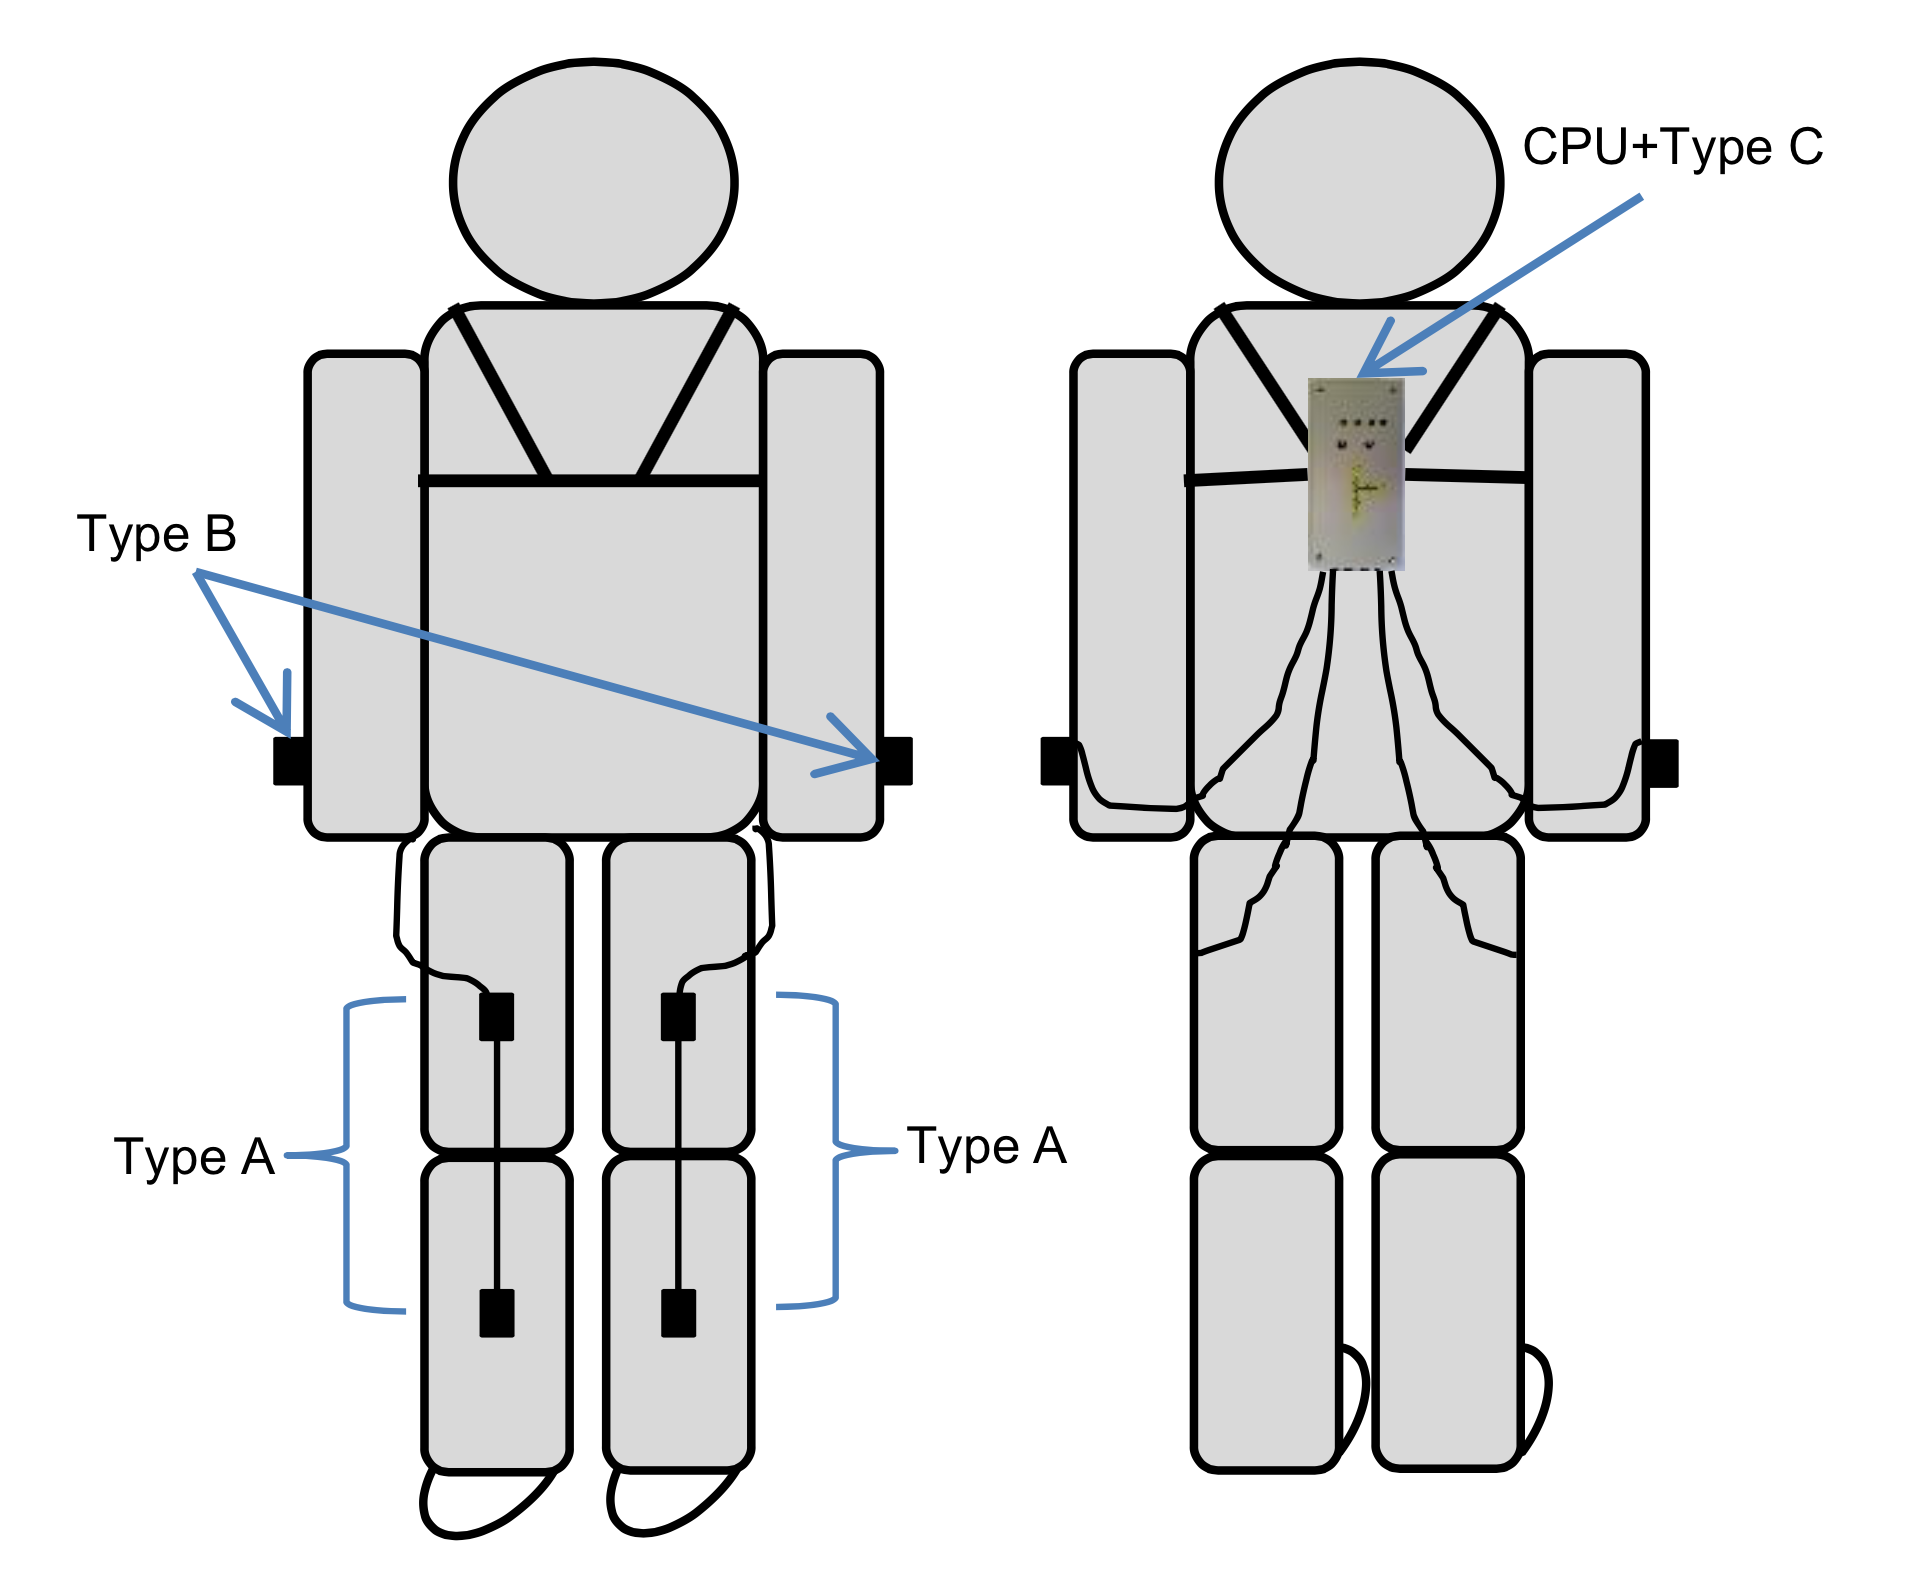
\includegraphics[width=10cm]{images/GaitWatch_placement}} at (0pt,0pt);
    \node [] (a) at (-4.4, -2) {Type A};
    \node [] (b) at (-4.5, 0.1) {Type B};
    \node [] (c) at (4.45, 3.25) {Type C};
\end{tikzpicture}
\caption{Placement of the GaitWatch components at the body, from \cite{olivares_vicente_gaitwatch_2013}.}
	\label{fig:GaitWatch_placement}
\end{figure}






	\chapter{Orientation Estimation Using MARG Sensors}
\label{ch:orientation_estimation}

This chapter covers the working principals of MARG sensors, as well as the fundamentals of orientation estimation, that are necessary for the implementation of the aforementioned system. Subsequently, a mathematical construct used to express orientation -- Euler angles -- is explained. Towards the end of the chapter, different approaches to compute orientation estimates from magnetic and inertial data including their pros and cons are described. Finally, sensor fusion as a means to mitigate the drawbacks of each approach is introduced.

\section{MARG Sensors}

MARG sensors is a collective term for magnetic, angular rate, and gravitational sensors, which encompasses inertial sensors, as well as magnetic field sensors, also referred to as magnetometers. Inertial sensors itself generally fall into two categories: instruments sensing linear inertial displacement, i.\,e. accelerometers, and rotational inertial rate sensors, that is gyroscopes. They are applied in various contexts to quantify vibration, motion, and shock \cite{bhattacharyya_inertial_sensors_applications_13}. Particularly, the development of \gls{MEMS} opened up many medical applications as stated in Section \ref{sec:MARG_sensors_medical}. MEMS sensors have low manufacturing costs, small physical size, and low power consumption \cite{bhattacharyya_inertial_sensors_applications_13}. This section compiles the functional principles of different MARG sensors and introduces \glspl{IMU} as a combination of those.

\subsection{Accelerometers}\label{sec:accelerometers}

Accelerometers measure the acceleration of an object relative to an inertial frame. Since acceleration cannot be sensed directly, the force exerted on a reference mass is measured. The resultant acceleration is computed according to Newton's second law $\mathbf{f} = m \cdot \mathbf{a}$, where $\mathbf{f} \in \mathbb{R}^3$ denotes the force vector, $m$ the mass, and $\mathbf{a} \in \mathbb{R}^3$ the acceleration vector. Usually, a single axis accelerometer consists of a small proof mass connected via a spring to the case of the instrument. The proof mass is displaced  by $\Delta x$ with respect to the case, when the instrument experiences a certain acceleration along its sensitive axis. Disregarding drag force, according to Hooke's law $f = -k \cdot \Delta x$, the displacement is directly proportional to the force exerted by the mass and thus to the acceleration. Therefore, by measuring the displacement of the proof mass the acceleration can be obtained. Figure \ref{fig:accelerometer} shows the displacement $\Delta x$ of the mass with respect to the case of the instrument for three different conditions: (a) at rest or in uniform motion, (b) accelerating, and (c) at rest, being exposed to the gravity $ \mathbf{g}$. According to how the mass displacement is sensed, accelerometers can be classified as resistive, capacitive, and piezoelectric. Besides, there are surface acoustic wave, fibre optic, vibrating beam and solid-state \gls{MEMS} accelerometers. To obtain a three-dimensional accelerometer, three single-axis accelerometers are mounted together. Nowadays, most accelerometers are manufactured using MEMS technology, which was developed for the military and aerospace markets in the 1970s \cite{bhattacharyya_inertial_sensors_applications_13}. 

\begin{figure}
\centering
\begin{tikzpicture}[scale=0.95, auto, thick, node distance=3cm,>=latex']
    \pgftext{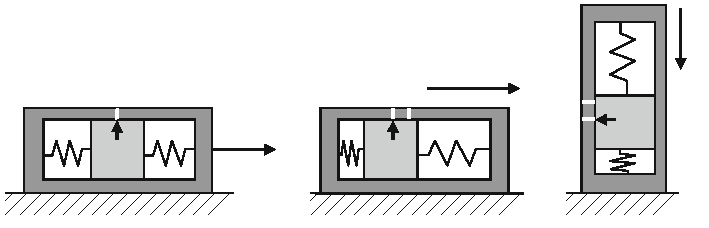
\includegraphics[width=13.5cm]{Figures/accelerometer}} at (0pt,0pt);
    \node [] (a) at (-6.7, -1.1) {(a)};
    \node [] (b) at (-1.1, -1.1) {(b)};
    \node [] (c) at (3.9, -1.1) {(c)};
    \node [] (c) at (-4.525, 0.44) {$0$};
    \node [] (c) at (1.03, 0.44) {$0$};
    \node [] (c) at (4, 0.26) {$0$};
    \node [] (c) at (0.58, 0.44) {$\Delta x$};
    \node [] (c) at (3.82, -0.08) {$\Delta x$};
    \node [] (c) at (6.5, 1.5) {$\mathbf{g}$};
    \node [] (c) at (-4.525, -0.75) {\scriptsize Proof};
    \node [] (c) at (-4.525, -1.05) {\scriptsize mass};
    \node [] (c) at (-2, -0.05) {\scriptsize Sensitive};
    \node [] (c) at (-2, -0.45) {\scriptsize axis};
    \node [] (c) at (2.2, 0.82) {$\mathbf{a}$};
\end{tikzpicture}
\caption{A mass-and-spring accelerometer under different conditions: (a) at rest or in uniform motion, (b) accelerating, and (c) at rest, being exposed to the gravity $\mathbf{g}$, from \cite{bhattacharyya_inertial_sensors_applications_13}.}
	\label{fig:accelerometer}
\end{figure}


\subsection{Gyroscopes}

Gyroscopes are used for measuring and maintaining angular orientation. In essence, based on two different physical principles, namely the Sagnac and Coriolis effect, gyroscopes sense angular velocity, which is why they are also referred to as angular velocity sensors or angular rate sensors. By integrating the angular velocity the rotation angle can be obtained. Here we will only elaborate on the working principle of vibrating gyroscopes, since they are utilised in the GaitWatch system. \citeauthor{armenise2010advances} give a comprehensive overview of current gyroscope technologies in \cite{armenise2010advances}.

Coriolis vibratory gyroscopes, or vibrating gyros for short, sense angular velocity based on the effect of Coriolis force on a vibrating mass. The Coriolis force is a fictitious force experienced by a mass $m$ moving in a rotating reference frame. It can be calculated as: $\mathbf{f}_C = -2m(\bm{\omega} \times \mathbf{v})$, where $\mathbf{v}$ is the mass velocity in the rotating reference frame and $\bm{\omega}$ is the angular velocity of the reference frame. As seen in this equation the Coriolis force is only present when the mass varies its distance with respect to the spin axis. Otherwise, if $\bm{\omega}$ and $\mathbf{v}$ are parallel, the cross product becomes zero. The two degree-of-freedom spring-mass-damper system shown in Figure \ref{fig:gyroscope} serves as a simple model of a vibrating angular rate sensor. The mass $m$ can move along the $x$ and $y$-axis, respectively. The angular velocity around the $z$-axis is denoted with $\omega$. The drive or primary oscillating mode, that is, the oscillation along $x$, is excited by the force $F_x$ directed along the $x$-axis. The oscillation along $y$, called sense or secondary oscillating mode, is due to system rotation around the $z$-axis. $D_x$ and $D_y$ are the damping coefficients and $k_x$ and $k_y$ are the spring constants along the $x$ and $y$-axis, respectively. Typically, the primary oscillating mode is excited by a sinusoidal force with an angular frequency close to the resonance frequency, so that $\Omega_x \cong \sqrt{k_x/m}$. Its amplitude is kept constant at $a_x$. As shown in \cite{armenise2010advances}, the amplitude of the sense mode is then given by

\begin{equation}
  a_y = -\frac{2 a_x \Omega_x \omega}{\sqrt{(\Omega^2_x - \Omega^2_y)^2 + \Omega^2_x \Omega^2_y / Q^2_y}}\,,
\end{equation}

\noindent
where $\Omega_y=\sqrt{k_y/m}$ is the resonance frequency of the secondary resonator and $Q_y = \sqrt{m k_y}/D_y$ its quality factor. The amplitude $a_y$ is directly proportional to the angular rate of the two degree-of-freedom spring-mass-damper system. Thus, $\omega$ can be estimated by measuring the amplitude of the oscillation along the $y$-axis.

Usually, vibrating gyroscopes are manufactured using MEMS technology. MEMS gyros are of low to medium accuracy \cite{bhattacharyya_inertial_sensors_applications_13}, but due to their size they are ideally suited for medical applications.

\begin{figure}
\centering
\begin{tikzpicture}[auto, thick,>=latex', cross/.style={path picture={ 
  \draw[black]
(path picture bounding box.south east) -- (path picture bounding box.north west) (path picture bounding box.south west) -- (path picture bounding box.north east); }}]

\tikzstyle{spring}=[thick,decorate,decoration={zigzag,pre length=0.3cm,post length=0.3cm,segment length=6}]
\tikzstyle{damper}=[thick,decoration={markings,  
  mark connection node=dmp,
  mark=at position 0.5 with 
  {
    \node (dmp) [thick,inner sep=0pt,transform shape,rotate=-90,minimum width=8pt,minimum height=7pt,draw=none] {};
    \draw [thick] ($(dmp.north east)+(4pt,0)$) -- (dmp.south east) -- (dmp.south west) -- ($(dmp.north west)+(4pt,0)$);
    \draw [thick] ($(dmp.north)+(0,-4pt)$) -- ($(dmp.north)+(0,4pt)$);
  }}, decorate]
\tikzstyle{ground}=[fill,pattern=north east lines,draw=none,minimum width=0.75cm,minimum height=0.3cm]


\node (M) [draw, minimum width=3cm, minimum height=3cm] {};

\node (ground) [ground,anchor=north,yshift=-1.5cm,minimum width=3.5cm] at (M.south) {};
\draw (ground.north east) -- (ground.north west);

\node (wall) [ground, rotate=-90, minimum width=3.5cm,yshift=-3cm] {};
\draw (wall.north east) -- (wall.north west);

\draw [spring] (wall.170) -- node [label={[label distance=-0.2cm]above:$k_x$}] {}($(M.north west)!(wall.170)!(M.south west)$);
\draw [damper] (wall.10) -- node [label={[label distance=-0.1cm]above:$D_x$}] {}($(M.north west)!(wall.10)!(M.south west)$);

\draw [spring] (ground.170) -- node [label={[label distance=0.09cm]right:$k_y$}] {}($(M.south east)!(ground.170)!(M.south west)$);
\draw [damper] (ground.10) -- node [label={[label distance=0.08cm]right:$D_y$}] {}($(M.south east)!(ground.10)!(M.south west)$);      

    \node[coordinate] (X) at (5,-1) {};
    \node[coordinate] (Y) at (3,1) {};
    \node[coordinate] (O) at (3, -1) {};
    
    \draw[->] (O) -- node[name=x] {$x$}(X);
    \draw[->] (O) -- node[name=y] {$y$}(Y);
    \node [draw,circle, fill=white,cross,minimum width=0.15 cm, label={[anchor=south west]below:$z$}](z) at (3, -1){};
    
    \draw[-stealth] (0.15,1) arc (80:390:1);
    
    \node at (0.6, 0.8) (angle1) {$\omega$};
    \node at (-1.05, 1.1) (angle1) {$m$};
    
    \draw [-stealth, align=center] (-0.5,2) -- node[name=Fx] {$F_x$} (0.5,2);

    
\end{tikzpicture}
\caption{A simple model of a Coriolis vibratory gyroscope: A two degree-of-freedom spring-mass-damper system in a rotating reference frame, from \cite{armenise2010advances}.} \label{fig:gyroscope}
\end{figure} 
 

\subsection{Magnetometers}

Magnetometers measure the strength and the direction of the magnetic field at a point in space. There are numerous techniques used to produce magnetic field sensors, which exploit a broad range of physical phenomena \cite{lenz_magnetic_2006}. \citeauthor{lenz_magnetic_2006} give a complete survey of common technologies used for magnetic field sensing in \cite{lenz_magnetic_2006}. Many \gls{MEMS} magnetometers sense mechanical motion of a MEMS structure due to Lorentz force and estimate the strength of the magnetic field according to the displacement. When an external magnetic field interacts with a current-carrying silicon MEMS structure the Lorentz force causes a displacement of this structure. Piezoresistive, capacitive, or optical sensing can be used to detect the displacement of the MEMS structure. MEMS Lorentz force magnetometers are free from hysteresis, require no specialised materials and can be monolithically integrated with other MEMS inertial sensors \cite{thompson_lorentz_2011}.

\section{Inertial Measurement Units}

Devices using a combination of accelerometers and gyroscopes to measure the orientation of a rigid body with up to six degrees of freedom are referred to as \glspl{IMU}. If they include additional magnetometers they are termed \glspl{MIMU}. The number of degrees of freedom states the number of independent motions, with respect to a reference frame that are allowed to the body in space. \glspl{MIMU} are portable and relatively inexpensive. They can be easily attached to the body and thus allow non-clinical longterm application. Their drawbacks are complex calibration procedures and drift behaviour over time, depending on intensity and duration of the measurement interval. Hence, in order to maintain a satisfactory degree of precision, periodical recomputation of the calibration parameters is required \cite{olivares_vicente_signal_2013}.

\section{Euler Angles}

As well as in aircraft navigation, in the motion monitoring field the position of the coordinate frame of the body, that is the \emph{body frame}, with respect to a reference coordinate frame, termed the \emph{world frame}, is known as \emph{attitude}, which is used as a synonym of orientation. \emph{Euler angles} are one of several mathematical ways to describe the attitude of an object in three-dimensional Euclidean space. They represent a sequence of three elemental rotations about the axes of the coordinate system, defined as follows:

\begin{itemize}
\item The \emph{roll} angle $\phi$ determines the rotation around the $x$-axis.
\item The \emph{pitch} angle $\theta$ determines the rotation around the $y$-axis.
\item The \emph{yaw} angle $\psi$ determines the rotation around the $z$-axis.
\end{itemize}

\noindent
Figure \ref{fig:Euler_angles} depicts the rotation about the axes $z, y', X$ by $\psi, \theta, \phi$, respectively, according to the Tait-Bryan convention. The colour blue indicates the world frame $\{x, y, z\}$, which matched the body frame $\{X, Y, Z\}$ before the rotations. The colour red indicates the orientation of the body frame after the rotations were carried out. In contrast to \emph{extrinsic rotations}, where each of the three elemental rotations may occur about the axes of the original coordinate system, the Tait-Bryan rotations are \emph{intrinsic rotations} that occur about the axes of the rotating coordinate system, which changes its orientation after each rotation.

\begin{figure}[t]
\centering
\begin{tikzpicture}[scale=1.4]
\node[inner sep=0pt] (tait) at (0,0)
    {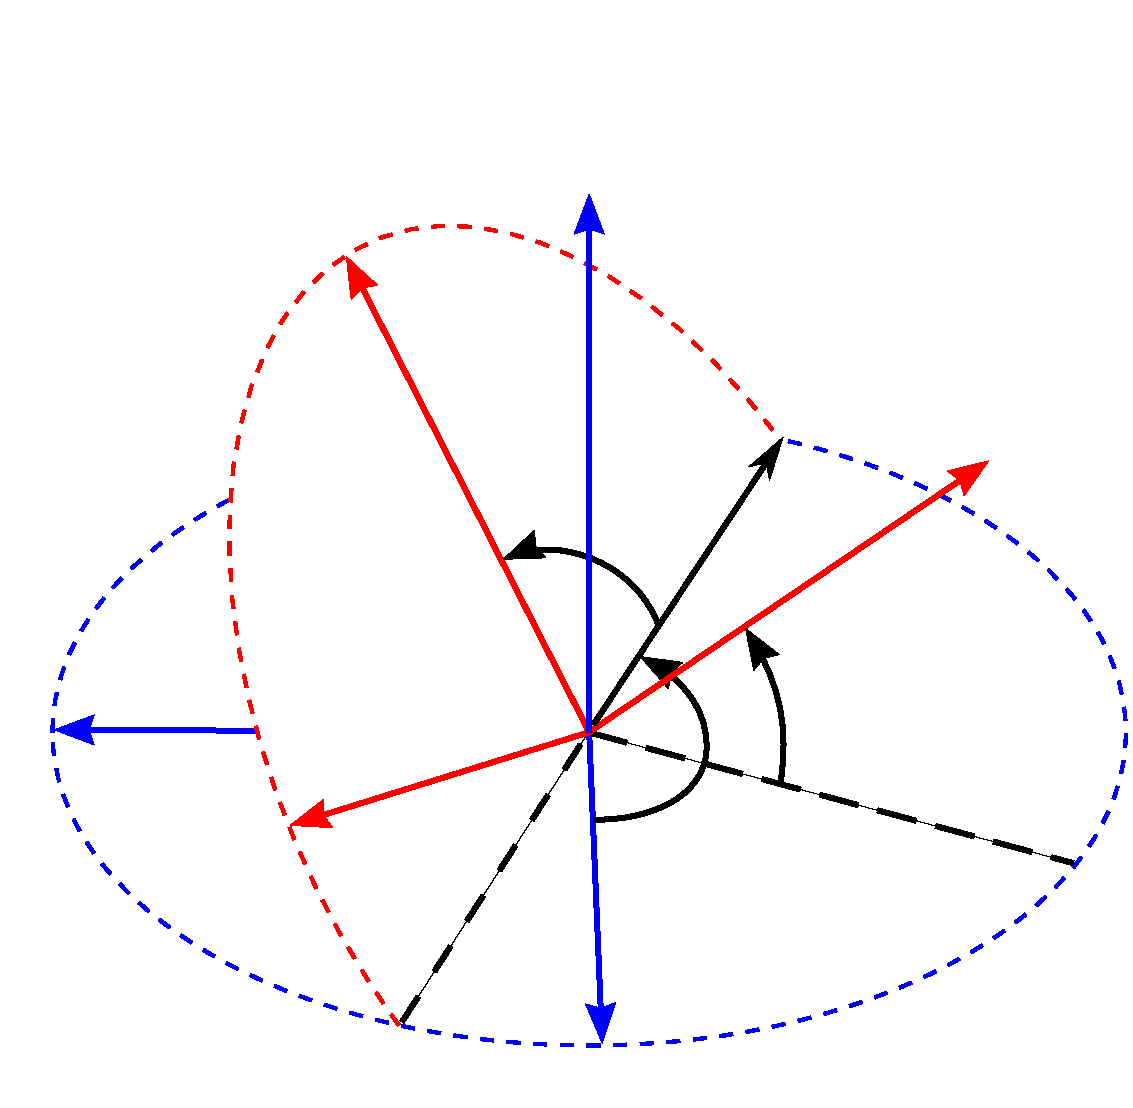
\includegraphics[width=.7\textwidth]{Figures/taitbryan.pdf}};
    
\node [] at (0.5,0.2) {$\phi$};
\node [] at (0.65,-1.85) {$\psi$};
\node [] at (1.55,-0.9) {$\theta$};

\node [] at (-3.4,-1.1) {$x$};
\node [] at (0.25,-3.3) {$y$};
\node [] at (0.12,2.43) {$z$};

\node [] at (1.5,1) {$y'$};
\node [] at (3.4,-1.9) {$x'$};
\node [] at (2.8,0.6) {$X$};
\node [] at (-1.5,2.05) {$Y$};
\node [] at (-2.0,-1.7) {$Z$};
\end{tikzpicture}
\caption{Representation of the body frame, depicted in red, with respect to the world frame, depicted in blue, from \cite{Wiki_taitbryan}. The body frame was rotated, by the Euler angles $\psi, \theta, \phi$ about the axes $z, y', X$, respectively.} \label{fig:Euler_angles}
\end{figure}

Euler angles are a simple and intuitive means to represent rotations in three-dimensional space. However, for the above mentioned parameterisation they have singularities at values of $\theta = n \pi$, $n \in \mathbb{Z}$. At these points a rotation about the $x$-axis and the $z$-axis constitute the same motion, which results in the loss of one degree of freedom and makes changes in $\phi$ and $\psi$ indistinguishable. This phenomenon is called \emph{gimbal lock}.

\subsection{Transformation Matrix}

Coordinates representing a point in one coordinate system can be transformed to another. Such a transformation can be expressed as a multiplication of a matrix with the coordinate vector that is to be transformed. Let $\mathbf{E}$ denote the orthonormal basis $\{x, y, z\} \in \mathbb{R}^3$ and let $\mathbf{E}'$ denote the orthonormal basis $\{X, Y, Z\} \in \mathbb{R}^3$. Furthermore, let $\mathbf{p}$ denote the position vector of an arbitrary point in three-dimensional Euclidean space. The coordinate transformation from $\mathbf{E}$ to $\mathbf{E}'$ is denoted $\bm{\Omega}_{\mathbf{E} \rightarrow \mathbf{E}'}: (p_1, p_2, p_3) \mapsto (p'_1, p'_2, p'_3)$. Then, the linear transformation from $\mathbf{p}$ to $\mathbf{p}'$ is given by

\begin{equation}\label{eq:transformation}
  \mathbf{p}' = \bm{\Omega}_{\mathbf{E} \rightarrow \mathbf{E}'}(\mathbf{p}) = \mathbf{T} \mathbf{p}\,,
\end{equation}

\noindent
where $\mathbf{T}$ is the \emph{transformation matrix}, which is a function of the rotation angles between the two coordinate systems.

In order to transform the coordinate vector from the \emph{world frame} to the \emph{body frame}, according to the common aerospace rotation sequence mentioned above and the \gls{NED} coordinate system, the transformation matrix $\mathbf{C}_{wb}$ is given by

\begin{equation}\label{eq:transformation_matrices}
\begin{split}
\mathbf{C}_{wb} & = \mathbf{T}_x(\phi) \mathbf{T}_y(\theta) \mathbf{T}_z(\psi) \\
 & = {\left[ \begin{smallmatrix}
    1 \; & 0 \; & 0 \\
    0 \; & \cos \phi \; & \sin \phi \\
    0 \; & -\sin \phi \; & \cos \phi
    \end{smallmatrix}\right]}
    {\bigg[ \begin{smallmatrix}
    \cos \theta \; & 0 \; & -\sin \theta \\
    0 \; & 1 \; & 0 \\
    \sin \theta \; & 0 \; & \cos \theta
    \end{smallmatrix} \bigg]}
    {\left[\begin{smallmatrix}
    \cos \psi \; & \sin \psi \; & 0 \\
    -\sin \psi \; & \cos \psi \; & 0 \\
    0 \; & 0 \; & 1
    \end{smallmatrix}\right]}\\
 & = {\left[\begin{smallmatrix}
   \cos \theta \cos \psi \; &
    \cos \theta \sin \psi \; &
   -\sin \theta \\
    \sin \phi \sin \theta \cos \psi - \cos \phi \sin \psi \;\; &
    \sin \phi \sin \theta \sin \psi + \cos \phi \cos \psi \;\; &
    \sin \phi \cos \theta \\
    \cos \phi \sin \theta \cos \psi + \sin \phi \sin \psi \;\; &
    \cos \phi \sin \theta \sin \psi - \sin \phi \cos \psi \;\; &
    \cos \phi \cos \theta
  \end{smallmatrix}\right]}
\end{split}
\end{equation}

\noindent
Plugged in Equation \ref{eq:transformation} ($\mathbf{T} = \mathbf{C}_{wb}$), the pre-multiplications of the matrices $\mathbf{T}_x(\phi), \mathbf{T}_y(\theta), \mathbf{T}_z(\psi)$ to the vector $\mathbf{p}$ represent the coordinate rotations about the single axes $x, y', Z$, according to the right hand rule, respectively. That is, the function $\bm{\Omega}_{\mathbf{E} \rightarrow \mathbf{E}'}$ maps the vector $\mathbf{p}$ to its orthogonal projection onto the axes of the coordinate system, $\mathbf{p}'$, which result from the respective two-dimensional rotation of $\phi, \theta, \psi$ about the axes $x, y', Z$. This is illustrated for a single rotation around the $z$-axis by the angle $\psi$ in Figure \ref{fig:transformation_matrix}. Note that $\{x', y', z'\}$ denotes the coordinate frame after the first elemental rotation. The matrices $\mathbf{T}_x(\phi), \mathbf{T}_y(\theta)$, and $\mathbf{T}_z(\psi)$ are also known as direction cosine matrices, since their elements are the cosines of the unsigned angles between the body-fixed axes and the axes of the world frame, as shown in \cite{diebel2006attitude}. The form stated here is already simplified. The matrix $\mathbf{C}_{bw}$ that transforms a coordinate vector from the body frame to the world frame is given by

\begin{figure}[t]
\centering

\tdplotsetmaincoords{60}{110}

\begin{tikzpicture}[scale=6,tdplot_main_coords]

\coordinate (O) at (0,0,0);
\pgfmathsetmacro{\psivec}{55}
\tdplotsetcoord{P}{0.8}{44}{\psivec}

\draw[thick,->] (0,0,0) -- (.8,0,0) node[anchor=north west]{$x$};
\draw[thick,->] (0,0,0) -- (0,.8,0) node[anchor=north west]{$y$};

\tdplotsetrotatedcoords{0}{0}{25}

\draw[thick,blue,tdplot_rotated_coords,->] (0,0,0) -- (.8,0,0) node[anchor=north west]{$x'$};
\draw[thick,blue,tdplot_rotated_coords,->] (0,0,0) -- (0,.8,0) node[anchor=west]{$y'$};
\draw[very thick,blue,tdplot_rotated_coords] (0,0,0) -- (0, 0.25, 0) node[anchor=south east]{$p_y'$};
\draw[thick,blue,tdplot_rotated_coords,->] (0,0,0) -- (0,0,.8) node[anchor=north west]{$z'=z$};
\draw[very thick,blue,tdplot_rotated_coords] (0,0,0) -- (0.507, 0, 0) node[pos=0.9, label={left:$p_x'$}, rounded corners=1pt]{};
\draw[very thick,blue,tdplot_rotated_coords] (0,0,0) -- (Pz) node[pos=0.5, label={left:$p_z'$}]{};

%draw a vector from origin to point (P) 
\draw[-stealth,color=red] (O) -- node [anchor=south]{$p$}(P);

%draw projection on xy plane, and a connecting line
\draw[dashed, red] (O) -- (Pxy);
\draw[dashed, red] (P) -- (Pxy);
\draw[dashed] (Px) -- (Pxy);
\draw[dashed] (Py) -- (Pxy);

\tdplotdrawarc[-stealth]{(0,0,0)}{0.58}{0}{25}{anchor=north}{$\psi$}

\draw[dashed] (0.8,0,0) arc (0:115:0.8);

\draw[dashed, blue, tdplot_rotated_coords] (0.507, 0, 0) -- (Pxy);
\draw[dashed, blue, tdplot_rotated_coords] (0, 0.25, 0) -- (Pxy);
\draw[dashed, blue, tdplot_rotated_coords] (P) -- (Pz);

\end{tikzpicture}
\caption{An exemplary coordinate rotation about the $z$-axis by an angle $\psi$, illustrating the orthogonal projection on the resulting axes $x', y', z'$.}
	\label{fig:transformation_matrix}
\end{figure}


\begin{equation}
\mathbf{C}_{bw} = {\left[\begin{smallmatrix}
   \cos \theta \cos \psi \; &
    \sin \phi \sin \theta \cos \psi - \cos \phi \sin \psi \; &
    \cos \phi \sin \theta \cos \psi + \sin \phi \sin \psi \\
    \cos \theta \sin \psi \;\; &
    \sin \phi \sin \theta \sin \psi + \cos \phi \cos \psi \;\; &
    \cos \phi \sin \theta \sin \psi - \sin \phi \cos \psi \\
    -\sin \theta \;\; &
    \sin \phi \cos \theta \;\; &
    \cos \phi \cos \theta
  \end{smallmatrix}\right]}
\end{equation}

\noindent
Note that $\mathbf{C}_{bw} = \mathbf{C}^T_{wb} = \mathbf{C}^{-1}_{wb}$. Thus, $\mathbf{C}^{ }_{bw}$ and $\mathbf{C}_{wb}$ are orthogonal matrices so that $\mathbf{C}^{ }_{bw} \mathbf{C}_{wb} = \mathbf{I}_3$, where $\mathbf{I}_3 \in \mathbb{R}^{3 \times 3}$ is the identity matrix.

\section{Projection of the Gravity Vector}\label{sec:projection_gravity}

% and Earth's Magnetic Field Vector

As described in Section \ref{sec:accelerometers}, accelerometers measure the linear acceleration they experience. Under static or quasi-static conditions, that is, the sensor is in uniform motion, or at low acceleration, it can be assumed that the measured acceleration is mainly that of gravity. By means of simple trigonometric functions estimates for the pitch and the roll angle can be obtained. Since the gravity vector is perpendicular to the $xy$-plane, and thus a rotation around the $z$-axis will not cause any variation in the sensed acceleration, the yaw angle cannot be obtained by this method. To solve this problem a three-dimensional magnetometer is used, which measures the variation of Earth's magnetic field while rotating around the $z$-axis.

When the accelerometer is motionless, its measurements will be directly related to the angle of the sensor relative to gravity, as depicted in Figure \ref{fig:acceleration_motion} (a). In that case $\theta$ with respect to the vertical is given by

\begin{equation} \label{eq:projection_gravity}
  \theta = \mbox{atan}2(A_z, A_x)\,,
\end{equation}

\noindent
where $A_x$ and $A_z$ are the components of the acceleration vector in $x$ and $z$-direction, respectively. However, when the sensor is in motion, in addition to the gravity, there are radial and tangential acceleration components due to motion, as depicted in Figure \ref{fig:acceleration_motion} (b). The magnitude of the gravity vector $\mathbf{g}$ is denoted with $\|\mathbf{g}\|$. Ignoring these components will cause incorrect angle estimates.

\begin{figure}
\centering
\resizebox{12.5cm}{!}{
\begin{subfigure}[]{0.45\textwidth}
\caption{}
\begin{tikzpicture}[auto, thick, node distance=3cm,>=latex']
    \node [draw, very thick, rounded corners=1pt, rectangle, minimum height=6em, minimum width=3em, align=center, rotate around={27:(-1,0.5)}] (sensor) {Sensor};
    \node[coordinate] (A) at (0.7, -0.6) {};
    \node[coordinate] (B) at (1.95, -3) {};
    \node[coordinate] (C) at (0.7, -3.56) {};
    
    \draw[->] (A) -- node[name=x] {$A_x = \|\mathbf{g}\| \cos \theta$}(B);
    \draw[->] (B) -- node[name=y] {$A_z = \|\mathbf{g}\| \sin \theta$}(C);
    \draw[->, very thick] (A) -- node[name=g, label={left:$\mathbf{g}$}] {}node [pos=0.35]{$\theta$} (C);
  
 	\draw[-stealth] (0.7,-2.0) arc (270:297:1.4);
      
    \end{tikzpicture}
\end{subfigure}
\quad
\begin{subfigure}[]{0.45\textwidth}
\caption{}
\begin{tikzpicture}[auto, thick, rounded corners=1pt, node distance=3cm,>=latex']
    \node [draw, very thick, rectangle, minimum height=6em, minimum width=3em, align=center, rotate around={27:(-1,0.5)}] (sensor) {Sensor};
    \node[coordinate] (A) at (0.7, -0.6) {};
    \node[coordinate] (B) at (2.1, -3.55) {};
    \node[coordinate] (C) at (0.7, -3.56) {};
    \node[coordinate] (D) at (1.2, -4) {};
    
    \draw[->, red, very thick] (A) -- node[name=d] {} (D);
    \draw[->] (A) -- node[name=x] {$A_x = A_{rad} + \|\mathbf{g}\| \cos \theta$} node [pos=0.46, label={left:$\theta$}]{} (B);
    \draw[->] (B) -- node[name=y] {$A_z = A_{tan} + \|\mathbf{g}\| \sin \theta$} (D);
    \draw[->, very thick] (A) -- node[name=g, label={left:$\mathbf{g}$}] {}(C);
      
    \draw[-stealth] (0.953,-2.2) arc (270:304:0.8);  
      
    \end{tikzpicture}	
\end{subfigure}
}
\caption{Acceleration seen by the sensor (b) with and (a) without motion, from \cite{bennett_motion_2014}.} \label{fig:acceleration_motion}
\end{figure} 

\section{Integration of the Angular Rate}\label{sec:integration_angular}

Another way to estimate the attitude of an object is the integration of the angular rate around the $x, y$ and $z$-axis, respectively. Although this would theoretically lead to very accurate orientation estimates, they are impaired by \gls{ARW} and dynamical bias in practice. \gls{ARW} is an effect caused by the integration of high-frequency, thermo-mechanical noise, which leads to a random additive angle in the orientation signal. An even greater impact than AWR has the gyroscope's dynamic bias, which has its origin in low-frequency flicker noise. Both effects cause a dramatical drift in the angle signal over time.

\section{Sensor Fusion}

Since the projection of the gravity vector is only valid under static or quasi-static conditions, or at low acceleration, and the integration of the angular rate leads to non-reliable estimates due to \gls{ARW} and dynamic bias, but is not affected by the intensity of motion, a means to combine the information of both sensors is desirable. The combination of information from multiple sensors to increase the overall precision of the estimation of a certain quantity of interest is termed \emph{sensor fusion}. \citeauthor{raol2009multi} \cite{raol2009multi} states the following advantages of sensor fusion:
 
\begin{itemize}
\item Robust functional and operational performance is given, in case of data loss from one sensor, due to redundancy provided by multiple sensors.
\item Enhanced confidence in the results inferred from the measurement of one sensor, if they are confirmed by the measurement of another sensor.
\item With sensor fusion an arbitrary fine time resolution of measurements is possible, whereas single sensors need a finite time to transmit measurements and so limit the frequency of measurements.
\item One sensor might be, to some extent, better in a certain state of the measured process, e.\,g. low or high motion intensity in attitude estimation, and thus, by fusing multiple sensor signals, a satisfactory accuracy among all states of the process could be attained.
\end{itemize}

\noindent
Sensor fusion can be realised by the use of a Kalman filter. This specific digital filter is described in detail in the next chapter, and applied in Chapter \ref{ch:Implementation} to fuse the sensor signals of accelerometers and gyroscopes.



	\chapter{Digital Filters}
\label{ch:kalman}

This Chapter dicusses basics of digital filters. The 
the shortcomings of the Wiener filter and its solution - the Kalman Filter a

In contrast to analogue filters that consist of electronic circuits to attenuate unwanted frequencies in continuous-time signals and thus extracted the useful signal, a digital filter is a set of mathematical operations applied to a discrete-time signal in order to extract information about the hidden quantity of interest. A sequence of samples at equidistant time instants represent the continuous-time signal with no loss, provided the sampling theorem is satisfied, according to which the sample frequency has to be greater than twice the highest frequency component of the continuous-time signal.

Digital filters can be classified as linear and nonlinear. If the quantity at the output of the filter is a linear function of its input, that is, the filter function satisfies the superposition principle, the filter is said to be linear. Otherwise, the filter is nonlinear.

\section{The Filtering Problem}

Conceived in general terms, a filter is a physical device for removing unwanted components of a mixture. In the technical field a filter is a system designed to extract information from noisy, distorted data. That is, the filter delivers an estimate of the variables of principal interest, which is why it may also be called an estimator. Filter theory is applied in diverse fields of science and technology, such as communications, radar, sonar, navigation, and biomedical engineering \cite{haykin2002adaptive}.

Consider, as an example involving filter theory, the continuous-time dynamical system depicted in Figure \ref{fig:state_estimation}. The desired state vector of the system, \gls{not:x(t)_v}, is usually hidden and can only be observed by indirect measurements \gls{not:y(t)_v} that are a function of \gls{not:x(t)_v} and subject to noise. Equally, the equation describing the evolution of the state \gls{not:x(t)_v} is usually subject to system errors. The dynamical system may be an aircraft in flight, in which case the elements of the state vector are constituted by its position and velocity. The measuring system may be a tracking radar producing the observation vector \gls{not:y(t)_v} over an interval $[0, T]$. The requirement is to deliver a reliable estimate \gls{not:x_hat(t)_v} of the state \gls{not:x(t)_v}, taking prior information into account.

\tikzstyle{block} = [draw, rectangle, minimum height=3em, minimum width=6em]
\tikzstyle{output} = [coordinate]
\tikzstyle{pinstyle} = [pin edge={to-, thin, black}, align=center]

\begin{figure}
\centering
\begin{tikzpicture}[auto, node distance=3cm,>=latex']
    \node [block, align=center, 
    	pin={[pinstyle]below:System \\ Errors}]
    	(dynamical) {Dynamical \\ system};
    \node [block, align=center, right of=dynamical, pin={[pinstyle]below:Measurement \\ errors}, node distance=4.5cm] (measuring) {Measuring \\ system};
    \node [block, align=center, right of=measuring, pin={[pinstyle]below:Prior \\ information}, node distance=4.5cm] (estimator) {Estimator};
    \node [output, right of=estimator] (output) {};
    
    \draw [->, align=center] (dynamical) -- node[name=x] {State \\ \gls{not:x(t)_v}} (measuring);
    \draw [->, align=center] (measuring) -- node[name=y] {Observation \\ \gls{not:y(t)_v}} (estimator);
    \draw [->, align=center] (estimator) -- node[name=y] {Estimate \\ of state \\ $\hat{\mathbf{x}}(t)$} (output);
\end{tikzpicture}
\caption{Block diagram depicting the components involved in state estimation adopted from \cite{haykin2002adaptive}.} \label{fig:state_estimation}
\end{figure}

\section{Wiener Filter}

A statistical criterion according to which the performance of a filter can be measured is the mean-squared error, defined as:

$$\operatorname{MSE}=\frac{1}{n}\sum_{i=1}^n(\hat{x}_i - x_i)^2$$

\noindent
where $i$ denotes the element of the vector  $\hat{\mathbf{x}}$ and the actual state vector $\mathbf{x}$ with a length of $n$, respectively. Assuming a stationary stochastic process with known statistical parameters as the mean and correlation functions of the useful signal and the unwanted additive noise, the so-called Wiener filter is said to be optimum as it minimises the mean-square value of the error signal. Since the Wiener filter requires apriori information about the statistics of the data to be processed, it may not be optimum for non-stationary processes.

\section{Adaptive Filters}

 

\section{Kalman Filter}

The following simple example from \cite{Maybeck79} is no complete mathematical derivation but an illustrative description of the determination of a one-dimensional position to understand how the Kalman filter works.

Suppose you are lost at sea during the night and take a star sighting to determine your approximate position at time $t_1$ to be $z_1$. Your location estimate is, due to inherent measurement device inaccuracies and human error, somewhat uncertain, and thus assumed to be associated with a standard deviation is $\sigma_{z_1}$. The conditional probability of $x(t_1)$, your actual position at time $t_1$, conditioned on the observed value $z_1$, is depicted in Figure 

\begin{tikzpicture}

\draw[thick] plot[samples=200, smooth, domain=-.5:5.5] (\x, {0.1+2.8/(0.9*sqrt(2*pi))*exp(-((\x-2.5)^2)/(2*0.9^2))}) coordinate[pos=0.8] (A);
  \draw[->] (-1,0) -- (6,0) node[right] {$x$};
  \draw[->] (0,-1) -- (0,2) node[right] {$f_{x(t_1)|z(t_1)}(x|z_1)$};
  
  
\end{tikzpicture}

\section{Extended Kalman Filter}



	\chapter{Implementation}
\label{ch:Implementation}

This chapter describes the theoretical design of the system and the implementation, based on the fundamentals acquired in the previous the chapters. Subsequently, the experiments and its results are presented.

\section{Initial Situation}

 (Any algorithms that are already implemented for comparison that I can cite or state and describe how they differ from the one that I will implement??)

\section{Theoretical Design}\label{sec:theoretical_design}

This section maps the theoretical design of the system proposed by \citeauthor{bennett_motion_2014} in \cite{bennett_motion_2014}, that is, the kinematic model and the extended Kalman filter, to the existing GaitWatch system and its associated conventions with respect to axes definitions and rotation about them. 

\subsection{Kinematic model}

When walking in a straight line, the human leg can be modelled as a two-link planar revolute robot \cite{bennett_motion_2014}. As depicted in Figure \ref{fig:robot}, the revolute joints of the \gls{pendubot} represent the hip und knee joint, and the two links the thigh and shank, respectively. The origin of the inertial navigation frame is located at the base of link 1, the upper of both links. The angle $\psi_1$ is measured with respect to the $x$-axis, and the angle $\psi_2$ of link 2, with respect to link 1.

\begin{figure}
\centering
\begin{tikzpicture}[auto, thick,>=latex']
	\node [draw, rectangle, minimum height=1.6cm, minimum width=1.6cm, pattern=north west lines] at (0,0) (solid) {};

    \node [draw,  fill=white, very thick, rectangle, rounded corners=3pt, minimum height=3.5cm, minimum width=1cm, align=center, rotate around={30:(0,0)}] at (0.7, -1.25) (link1) {};
    \node [draw, thick, fill=gray, rounded corners=2pt, rectangle, minimum height=0.8cm, minimum width=0.5cm, align=center, rotate around={30:(0, 0)}, label={[label distance=0.18cm]335:IMU 1}] at (0.98, -1.7) (sensor1) {};
    
    \node [draw, fill=white, very thick, rectangle, rounded corners=3pt, minimum height=3.5cm, minimum width=0.6cm, align=center, rotate around={145:(0,0)}] at (0.6, -3.7) (link2) {};
    \node [draw, thick, fill=gray, rounded corners=2pt, rectangle, minimum height=0.8cm, minimum width=0.5cm, align=center, rotate around={145:(0, 0)}, label={left:IMU 2}] at (0, -4.56) (sensor2) {};
    
    \node[coordinate] (X) at (2.5,0) {};
    \node[coordinate] (Y) at (0,2.5) {};
    \node[coordinate] (O) at (-0, 0) {};
    
    \draw[->] (O) -- node[name=x] {$x$}(X);
    \draw[->] (O) -- node[name=y] {$y$}(Y);
    \draw[dotted] (O) -- (2.5,-4.3);
    \draw[fill=white] (0,0) circle (4pt);
    \draw (1.45, -2.5) circle (4pt);
    
    \draw[-stealth] (1.2,-1) arc (300:355:1.2);
    \draw[-stealth] (0.8,-4.1) arc (240:303:1.4);
    
    \node at (1.3, -0.4) (angle1) {$\psi_1$};
    \node at (1.5, -3.7) (angle1) {$\psi_2$};

\end{tikzpicture}
\caption{Acceleration seen by the sensor attached to the pendubot (b) with and (a) without motion from \cite{bennett_motion_2014}.} \label{fig:robot}
\end{figure} 

The \glspl{IMU} on the thighs and shanks measured the angular velocity and linear acceleration of the thighs and shanks, respectively. According to \citeauthor{spong2005robot} \cite{spong2005robot}, the $x$ and $y$ displacement and the related derivatives in the world frame are

\begin{align}
  x &= a_1 \cos \psi_1 + a_2 \cos(\psi_1 + \psi_2) \\
  \dot{x} &= -a_1 \dot{\psi}_1 \sin \psi_1  - a_2 (\dot{\psi}_1 + \dot{\psi}_2) \sin(\psi_1 + \psi_2) \\
  \ddot{x} {}&= -a_1 [\dot{\psi}^2_1 \cos \psi_1 + \ddot{\psi}_1 \sin \psi_1] - a_2 [(\dot{\psi}_1 + \dot{\psi}_2)^2 \cos(\psi_1 + \psi_2) \nonumber \\ 
  &\mathrel{\phantom{=}} + (\ddot{\psi}_1 + \ddot{\psi}_2) \sin(\psi_1 + \psi_2)] \label{eq:acc_x} \\
  \nonumber \\
  y &= a_1 \sin \psi_1 + a_2 \sin(\psi_1 + \psi_2) \\
  \dot{y} &= a_1 \dot{\psi}_1 \cos \psi_1  + a_2 (\dot{\psi}_1 + \dot{\psi}_2) \cos(\psi_1 + \psi_2) \\
  \ddot{y} {}&= a_1 [\ddot{\psi}_1 \cos \psi_1 - \dot{\psi}^2_1 \sin \psi_1] + a_2 [(\ddot{\psi}_1 + \ddot{\psi}_2) \cos(\psi_1 + \psi_2) \nonumber \\ 
  &\mathrel{\phantom{=}} - (\dot{\psi}_1 + \dot{\psi}_2)^2 \sin(\psi_1 + \psi_2)] \label{eq:acc_y}
\end{align}

\noindent
in which $a_1$ and $a_2$ are the lengths of the two links, respectively.

The orientation of the sensor frames at rest are different from the world frame and dynamic when the pendulum is in motion. To transform the values from the world frame to the dynamic body frame of \gls{IMU} 2, which is depicted in Figure, we used the transformation matrix $\mathbf{T}_z(\psi)$ in Equation \ref{eq:transformation_matrices} with $\psi = \psi_1 + \psi_2$, which yields

\begin{equation}
\mathbf{T}_z(\psi) = \begin{bmatrix}
    \cos (\psi_1 + \psi_2) \; & \sin (\psi_1 + \psi_2) \; & 0 \\
    -\sin (\psi_1 + \psi_2) \; & \cos (\psi_1 + \psi_2) \; & 0 \\
    0 \; & 0 \; & 1
    \end{bmatrix}\,.
\end{equation}

\noindent
The rotated tangential and radial components of the motion based acceleration estimates, $A_{tan}$ and $A_{rad}$ are found using $\mathbf{T}_z(\psi)$ to rotate the results of Equations \ref{eq:acc_x} and \ref{eq:acc_y}, according to Equation \ref{eq:transformation}, respectively.

Then, the tangential and radial acceleration estimates are subtracted from the sensor readings $A_x$ and $A_y$, which leaves an estimate of the gravity based acceleration $\mathbf{g}$ that acts on the sensor:

\begin{equation}
\begin{bmatrix}
    g_x \\
    g_y 
    \end{bmatrix} = 
    \begin{bmatrix}
    A_x \\
    A_y 
    \end{bmatrix} -
    \begin{bmatrix}
    A_{rad} \\
    A_{tan} 
    \end{bmatrix}\,.
\end{equation}

\noindent
According to Equation \ref{eq:projection_gravity} the improved angle estimate is

\begin{equation}
  \theta = \mbox{atan2}(\frac{g_y}{g_x})\,.
\end{equation}

\noindent
This can be used to reduce the estimation error due to gyroscope drift.

\subsection{Extended Kalman Filter Model}

The state space model of the extended Kalman filter is given by the state vector

\begin{equation} \label{eq:state_vector}
  \mathbf{x} = \begin{bmatrix}
  	x, & y, & \psi_1, & \omega_1, & \alpha_1, & \psi_2, & \omega_2, & \alpha_2, & \beta_1, & \beta_2
  \end{bmatrix}^T
\end{equation}

where $\psi_1$ is the angle, $\omega_1$ the angular velocity, and $\alpha_1$ the angular acceleration of the first joint, respectively. The corresponding values for the second link are $\psi_2$, $\omega_2$, and $\alpha_2$. The biases from the gyroscope on the first and second sensor are $\beta_1$ and $\beta_2$, respectively. They are assumed to be constant or slowly time varying.

The measurement matrix $\mathbf{y}$ is given by

\begin{equation} \label{eq:measurement_vector}
  \mathbf{y} = \begin{bmatrix}
  	\omega_1 + \beta_1, & \omega_1 + \omega_2 + \beta_2, & \psi_1 + \psi_2
  \end{bmatrix}^T\,.
\end{equation}
 
\noindent
The element $y_1$ represents the measurement of the first link angular velocity, which is the sum of the first link rotation and the gyroscope 1 bias. Equally, the element $y_2$ represents the measurement of the second link angular velocity, which is the sum of the first and second link rotation and the bias of gyroscope 2. Finally, the element $y_3$ is the angle estimate of the second accelerometer, which will see the angular displacement of both links.

(As in 20 )The linear approximation of the state equations at each iteration yields the state transition matrix

\begin{equation}
  \bm{\Phi}^{[1]}_{k} =  \mathbf{I}_{10} + \mathbf{F} T_s\,,
\end{equation}

\noindent
with

\begin{equation}
\mathbf{F} = \begin{bmatrix}
  0 & 0 & 0 & A & 0 & 0 & B & 0 & 0 & 0\\
  0 & 0 & 0 & C & 0 & 0 & D & 0 & 0 & 0\\
  0 & 0 & 0 & 1 & 0 & 0 & 0 & 0 & 0 & 0\\
  0 & 0 & 0 & 0 & 1 & 0 & 0 & 0 & 0 & 0\\
  0 & 0 & 0 & 0 & 0 & 0 & 0 & 0 & 0 & 0\\
  0 & 0 & 0 & 0 & 0 & 0 & 1 & 0 & 0 & 0\\
  0 & 0 & 0 & 0 & 0 & 0 & 0 & 1 & 0 & 0\\
  0 & 0 & 0 & 0 & 0 & 0 & 0 & 0 & 0 & 0\\
  0 & 0 & 0 & 0 & 0 & 0 & 0 & 0 & 0 & 0\\
  0 & 0 & 0 & 0 & 0 & 0 & 0 & 0 & 0 & 0\\
\end{bmatrix}\,,
\end{equation}

\noindent
and

\begin{equation*}
  \begin{array}{cc}
  \begin{split}
  	A &= -a_1 \sin \psi_1 -a_2 \sin (\psi_1 + \psi_2)\,, \quad \\
  	C &= a_1 \cos \psi_1 + a_2 \cos (\psi_1 + \psi_2)\,,
  \end{split} &
  \begin{split}
  B &= -a_2 \sin (\psi_1 + \psi_2)\,, \\
  C &= a_2 \cos (\psi_1 + \psi_2)\,,	
  \end{split}
\end{array}
\end{equation*}

\noindent
where $T_s$ is the sampling period and $\mathbf{I} \in \mathbb{R}^{10 \times 10}$ the identity matrix.

\begin{equation}
\mathbf{H} = \begin{bmatrix}
  0 & 0 & 0 & 1 & 0 & 0 & 0 & 0 & 1 & 0\\
  0 & 0 & 0 & 1 & 0 & 0 & 1 & 0 & 0 & 1\\
  0 & 0 & 1 & 0 & 0 & 1 & 0 & 0 & 0 & 0\\
\end{bmatrix}\,.
\end{equation}

\begin{equation}
\mathbf{R} = \begin{bmatrix}
  \sigma_1 & 0 & 0\\
  0 & \sigma_2 & 0\\
  0 & 0 & \sigma_3
\end{bmatrix}\,.
\end{equation}

\begin{equation}
\mathbf{Q} = \begin{bmatrix}
  \sigma_d & 0 & 0 & 0 & 0 & 0 & 0 & 0 & 0 & 0\\
  0 & \sigma_d & 0 & 0 & 0 & 0 & 0 & 0 & 0 & 0\\
  0 & 0 & 0 & 0 & 0 & 0 & 0 & 0 & 0 & 0\\
  0 & 0 & 0 & 0 & 0 & 0 & 0 & 0 & 0 & 0\\
  0 & 0 & 0 & 0 & 0 & 0 & 0 & 0 & 0 & 0\\
  0 & 0 & 0 & 0 & 0 & 0 & 0 & 0 & 0 & 0\\
  0 & 0 & 0 & 0 & 0 & 0 & 0 & 0 & 0 & 0\\
  0 & 0 & 0 & 0 & 0 & 0 & 0 & 0 & 0 & 0\\
  0 & 0 & 0 & 0 & 0 & 0 & 0 & 0 & 0 & 0\\
  0 & 0 & 0 & 0 & 0 & 0 & 0 & 0 & 0 & 0\\
\end{bmatrix}\,.
\end{equation}

\section{Implementation}

The filter algorithm was implemented in \textsc{Matlab}$\textsuperscript{\textregistered}$.

\section{Experiments}

The movement data was gathered at the Department of Neurology of the Klinikum Großhadern, Munich.

\subsection{Test Sequence}

The subject wore the GaitWatch system on his body. Then, the following sequence was carried out by the patient: The subject stood in front of the force plate. Then, the GaitWatch and force plate record was started and the subject made a step onto the force plate. After standing upright for a variable time of two to ten seconds the subject left the force plate, made a few steps, turned left, and stopped in front of it again. This sequence was repeated ten times.

\section{Results}

\section{Discussion}


	\chapter{Conclusion and Future Work}
\label{ch:Conclusion and Future Work}

\section{Conclusions}

%Gait analysis is a useful tool both in clinical practice and biomechanical research. In order to replace motion capture systems with low cost wearable \gls{MARG} sensors detailed technical matters still need to be improved \cite{tao_gait_2012}.
%
%Summarising the above, I can say that I have learned a lot in the four month that I spent in Granada. Amongst others I have come to know many new work methods, not only due to being exposed to people from a different culture, but also due to the fact that scientific research differs strongly from the work as a student at university. I gained a deeper understanding of orientation estimation and how Kalman filtering improves those. Therefore I had to study the principles of Kalman filters as well as the basics of MARG sensors. I was able to improve my MATLAB$\textsuperscript{\textregistered}$ skills and have realised how important it is to write understandable and well commented code, if it is for a larger project and not only for a coursework. I am now familiar with tools such as GitHub and Pivotal Tracker which make working in a team much easier and significantly more efficient.  Beside my work at the research centre, where I obtained a valuable insight into scientific research, I read a book about scientific writing that helped me to improve my oral and written English skills during my stay. Furthermore I now know the fundamentals of \LaTeX{}.
%
%All in all it was a great experience, professionally as well as personally. I truly and unreservedly recommend such a stay to \emph{every} university student.

\section{Future Work}

%Medical engineering is a very interesting blend of both my major interests, that is, working in the medical field as a paramedic and  in the technical field as an electrical engineer. There is a variety of possible future work. One related topic would be the validation of the pitch angles measured with the gyroscopes of the GaitWatch by means of cameras that record the trace of visual markers. From these markers one could compute the pitch angels and compare them to the those of the GaitWatch.



	
	\clearemptydoublepage
	\bibliographystyle{unsrtnat}
	\addcontentsline{toc}{chapter}{Bibliography}
	\bibliography{Bibliography}
	\clearemptydoublepage
	
\end{document}
